\begin{center}
  \textbf{Отчёт лабораторной работы №\envReportLabNumber}
\end{center}

\textbf{Тема}:
<<\envReportTitle>>

\textbf{Цель}: приобрести навыки написания запросов выборки данных.

% = = = = = = = = = = = = = = = =

\begin{center}
  \textbf{Подготовка к лабораторной работе}
\end{center}

% Перед тем как начать делать эту лабораторную работу, нужно спроектировать базу данных до 3-ей нормальной формы
% и заполнить её данными, чтобы SELECT-ом получать данные.

% Базу данных до 3-ей нормальной формы спроектировали во 2-ой лабораторной работе.
Логическая модель базы данных спроектированная в SQL Power Architect изображена на рисунке~\ref{fig:database}.

\begin{figure}[!h]
  \centering

  \includegraphics[width=18cm]
  {../database/logic_model.architect.pdf}

  \caption{Логическая модель}

  \label{fig:database}
\end{figure}

% Я на Node JS написал код, который генерирует файл *.sql, которые содержит транзакции с INSERT-ами.
% Например таблицу с осмотрами я заполнял за три кода.
% Каждый рабочий день работаю несколько участков и врачи проводят прием либо в поликлинике, либо дома.

% Я заполнил следующие таблицы (СУБД Postgres) рандомными данными:

% \begin{itemize}
%   \item справочник <<Диагнозы>>, результат на рисунке~\ref{fig:DE_CTL_Diagnosis};
%   \item справочник <<Доктора>>, результат на рисунке~\ref{fig:DE_CTL_Doctors};
%   \item справочник <<Гендеры>>, результат на рисунке~\ref{fig:DE_CTL_Genders};
%   \item справочник <<Места осмотра>>, результат на рисунке~\ref{fig:DE_CTL_InspectionPlaces};
%   \item справочник <<Лекарства>>, результат на рисунке~\ref{fig:DE_CTL_Medicines};
%   \item справочник <<Пациенты>>, результат на рисунке~\ref{fig:DE_CTL_Patients};
%   \item справочник <<Симптомы>>, результат на рисунке~\ref{fig:DE_CTL_Symptoms};
%   \item оперативный документ <<Осмотр>>, результат на рисунке~\ref{fig:DE_DOC_Inspection};
%   \item табличная часть <<Лекарства выписанные при осмотре>>, результат на рисунке~\ref{fig:DE_TAB_InspectionMedicines};
%   \item табличная часть <<Симптомы выявленные при осмотре>>, результат на рисунке~\ref{fig:DE_TAB_InspectionSymptoms};
%   \item табличная часть <<Симптомы выявленные при осмотре>>, результат на рисунке~\ref{fig:DE_TAB_MedicineSideEffects}.
% \end{itemize}

% \begin{figure}[p!h]
%   \centering

%   \includegraphics[height=5cm]
%   {inc/DE_CTL_Diagnosis.png}

%   \caption{Справочник <<Диагнозы>>}

%   \label{fig:DE_CTL_Diagnosis}
% \end{figure}

% \begin{figure}[p!h]
%   \centering

%   \includegraphics[height=5cm]
%   {inc/DE_CTL_Doctors.png}

%   \caption{Справочник <<Доктора>>}

%   \label{fig:DE_CTL_Doctors}
% \end{figure}


% \begin{figure}[p!h]
%   \centering

%   \includegraphics[height=5cm]
%   {inc/DE_CTL_Genders.png}

%   \caption{Справочник <<Гендеры>>}

%   \label{fig:DE_CTL_Genders}
% \end{figure}

% \begin{figure}[p!h]
%   \centering

%   \includegraphics[height=5cm]
%   {inc/DE_CTL_InspectionPlaces.png}

%   \caption{Справочник <<Места осмотра>>}

%   \label{fig:DE_CTL_InspectionPlaces}
% \end{figure}

% \begin{figure}[p!h]
%   \centering

%   \includegraphics[height=5cm]
%   {inc/DE_CTL_Medicines.png}

%   \caption{Справочник <<Лекарства>>}

%   \label{fig:DE_CTL_Medicines}
% \end{figure}

% \begin{figure}[p!h]
%   \centering

%   \includegraphics[height=5cm]
%   {inc/DE_CTL_Patients.png}

%   \caption{Справочник <<Пациенты>>}

%   \label{fig:DE_CTL_Patients}
% \end{figure}

% \begin{figure}[p!h]
%   \centering

%   \includegraphics[height=5cm]
%   {inc/DE_CTL_Symptoms.png}

%   \caption{Справочник <<Симптомы>>}

%   \label{fig:DE_CTL_Symptoms}
% \end{figure}

% \begin{figure}[p!h]
%   \centering

%   \includegraphics[height=5cm]
%   {inc/DE_DOC_Inspection.png}

%   \caption{Оперативный документ <<Осмотры>>}

%   \label{fig:DE_DOC_Inspection}
% \end{figure}

% \begin{figure}[p!h]
%   \centering

%   \includegraphics[height=5cm]
%   {inc/DE_TAB_InspectionMedicines.png}

%   \caption{Табличная часть <<Лекарства выписанные при осмотре>>}

%   \label{fig:DE_TAB_InspectionMedicines}
% \end{figure}

% \begin{figure}[p!h]
%   \centering

%   \includegraphics[height=5cm]
%   {inc/DE_TAB_InspectionSymptoms.png}

%   \caption{Табличная часть <<Симптомы выявленные при осмотре>>}

%   \label{fig:DE_TAB_InspectionSymptoms}
% \end{figure}

% \begin{figure}[p!h]
%   \centering

%   \includegraphics[height=5cm]
%   {inc/DE_TAB_MedicineSideEffects.png}

%   \caption{Табличная часть <<Симптомы выявленные при осмотре>>}

%   \label{fig:DE_TAB_MedicineSideEffects}
% \end{figure}

% \newpage

\begin{center}
\textbf{Задание 1}
\end{center}

\textbf{Условие}:
Вывести данные о всех приемах (дату, продолжительность приема в минутах, место
осмотра, данные врача, данные пациента), которые были проведены между датами
01.01.19 и 20.02.19 (привести два варианта решения задачи).

\lstinputlisting[language=sql]{../sql/task1/1.sql}

\textbf{Время выполнения}: 109-189 msec.

\textbf{Размер выборки}: 11996 rows.

\textbf{Результат}: часть выборки (в скриншоте LIMIT 48) изображена на рисунке~\ref{fig:t1}.

\begin{figure}[!h]
  \centering

  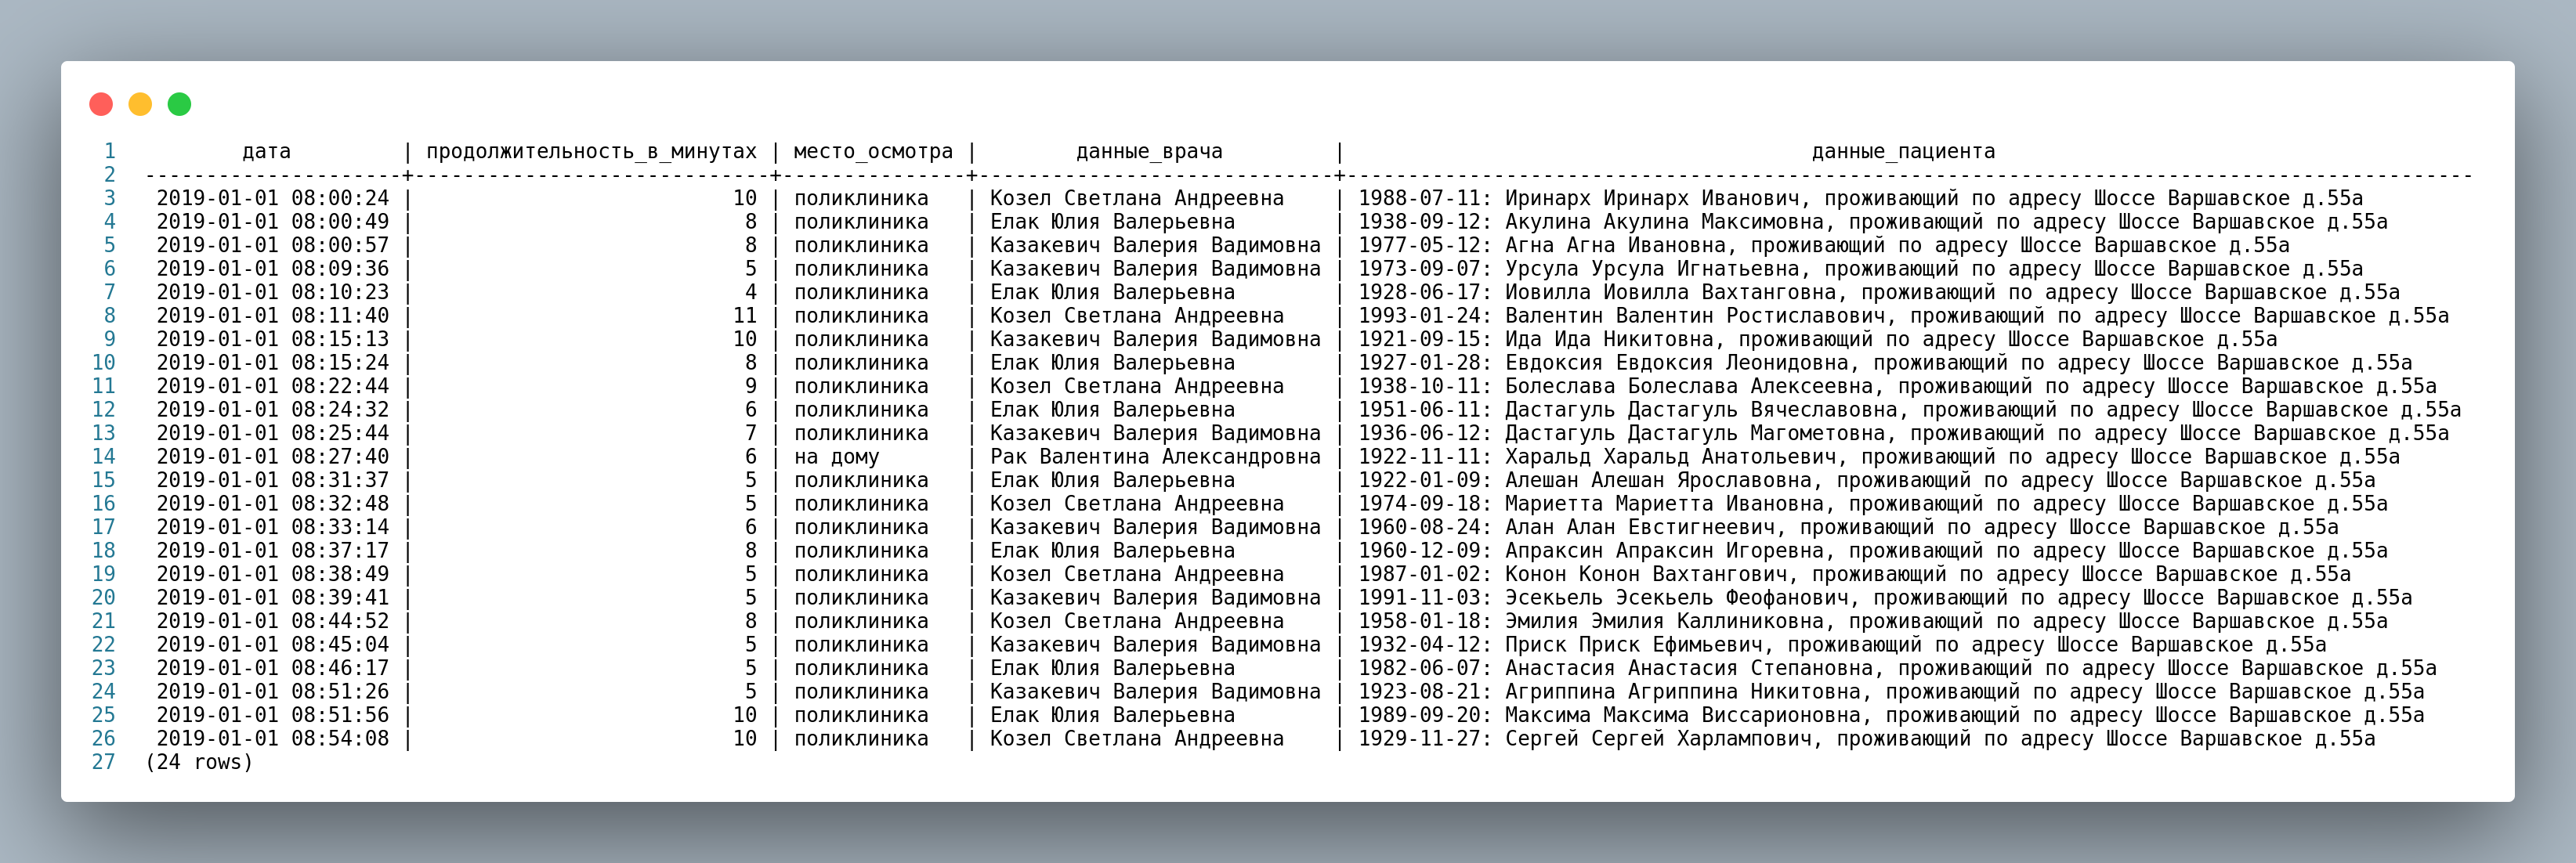
\includegraphics[width=18cm]
  {../sql/task1/1-out.png}

  \caption{Выборка из задания №1}

  \label{fig:t1}
\end{figure}

% = = = = = = = = = = = = = = = =

\newpage

\begin{center}
  \textbf{Задание 2}
\end{center}
  
\textbf{Условие}:
Вывести названия всех лекарств, у которых в названии присутствует '3\%'.

\lstinputlisting[language=sql]{../sql/task2/2.sql}

\textbf{Время выполнения}: 49-142 msec.

\textbf{Размер выборки}: 6 rows.

\textbf{Результат}: вся выборка изображена на рисунке~\ref{fig:t2}.

\begin{figure}[!h]
  \centering

  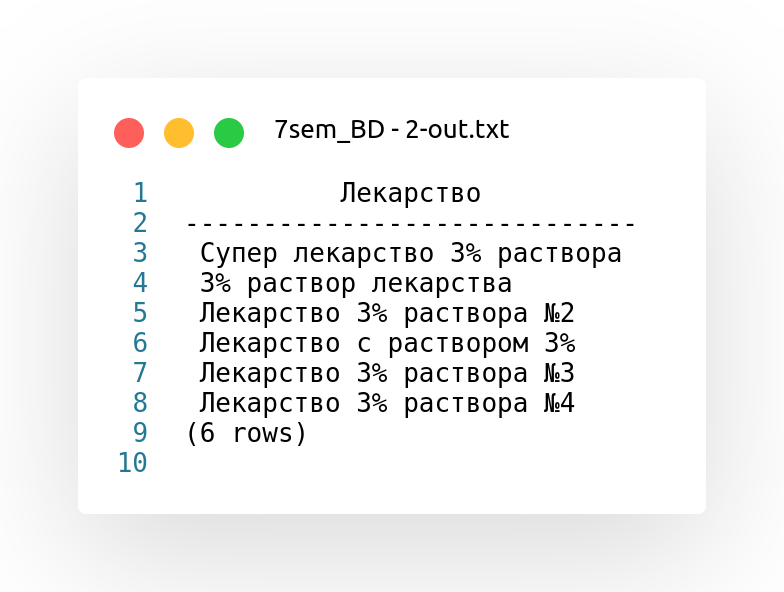
\includegraphics[height=5cm]
  {../sql/task2/2-out.png}

  \caption{Выборка из задания №2}

  \label{fig:t2}
\end{figure}

% = = = = = = = = = = = = = = = =

\begin{center}
  \textbf{Задание 3}
\end{center}
  
\textbf{Условие}:
Вывести данные о врачах, обслуживших максимальное количество пациентов на дому.

\lstinputlisting[language=sql]{../sql/task3/3.sql}

\textbf{Время выполнения}: 272-328 msec.

\textbf{Размер выборки}: 1 row.

\textbf{Результат}: вся выборка изображена на рисунке~\ref{fig:t3}.

\begin{figure}[!h]
  \centering

  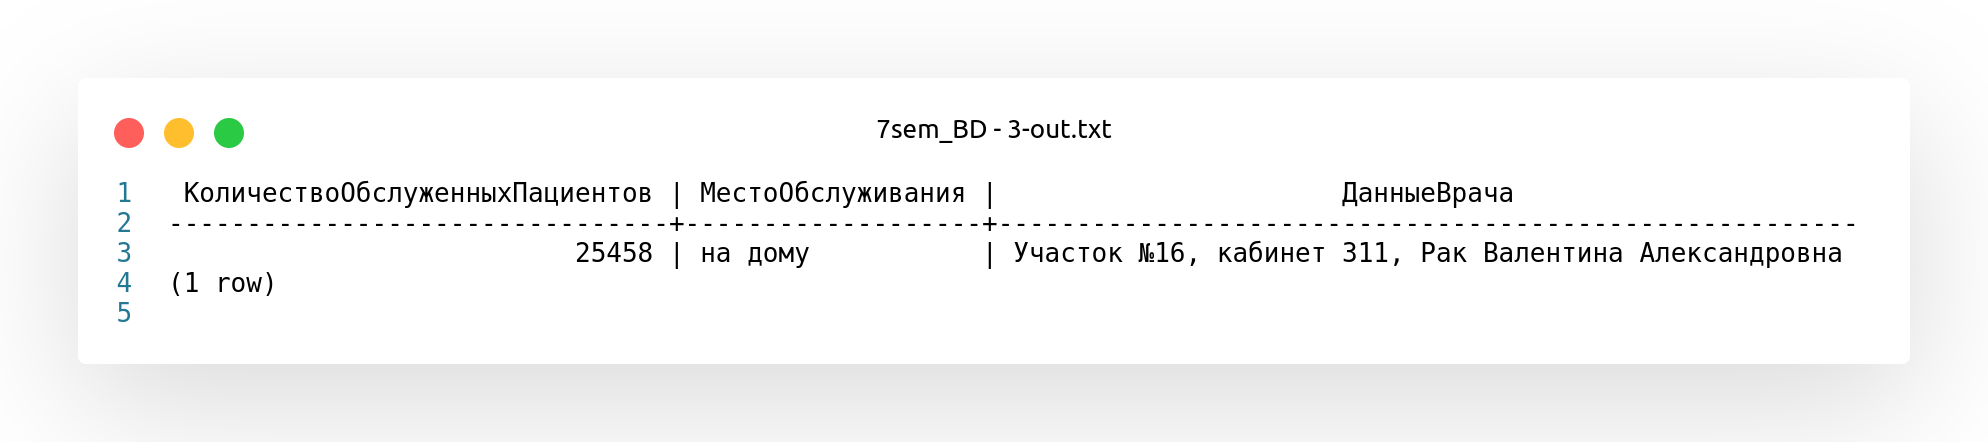
\includegraphics[width=18cm]
  {../sql/task3/3-out.png}

  \caption{Выборка из задания №3}

  \label{fig:t3}
\end{figure}

% = = = = = = = = = = = = = = = =

\newpage

\begin{center}
  \textbf{Задание 4}
\end{center}
  
\textbf{Условие}:
Для каждого врача подсчитать общее время обслуживания пациентов в госпитале.

\lstinputlisting[language=sql]{../sql/task4/4.sql}

\textbf{Время выполнения}: 113-170 msec.

\textbf{Размер выборки}: 14 rows.

\textbf{Результат}: вся выборка изображена на рисунке~\ref{fig:t4}.

\begin{figure}[!h]
  \centering

  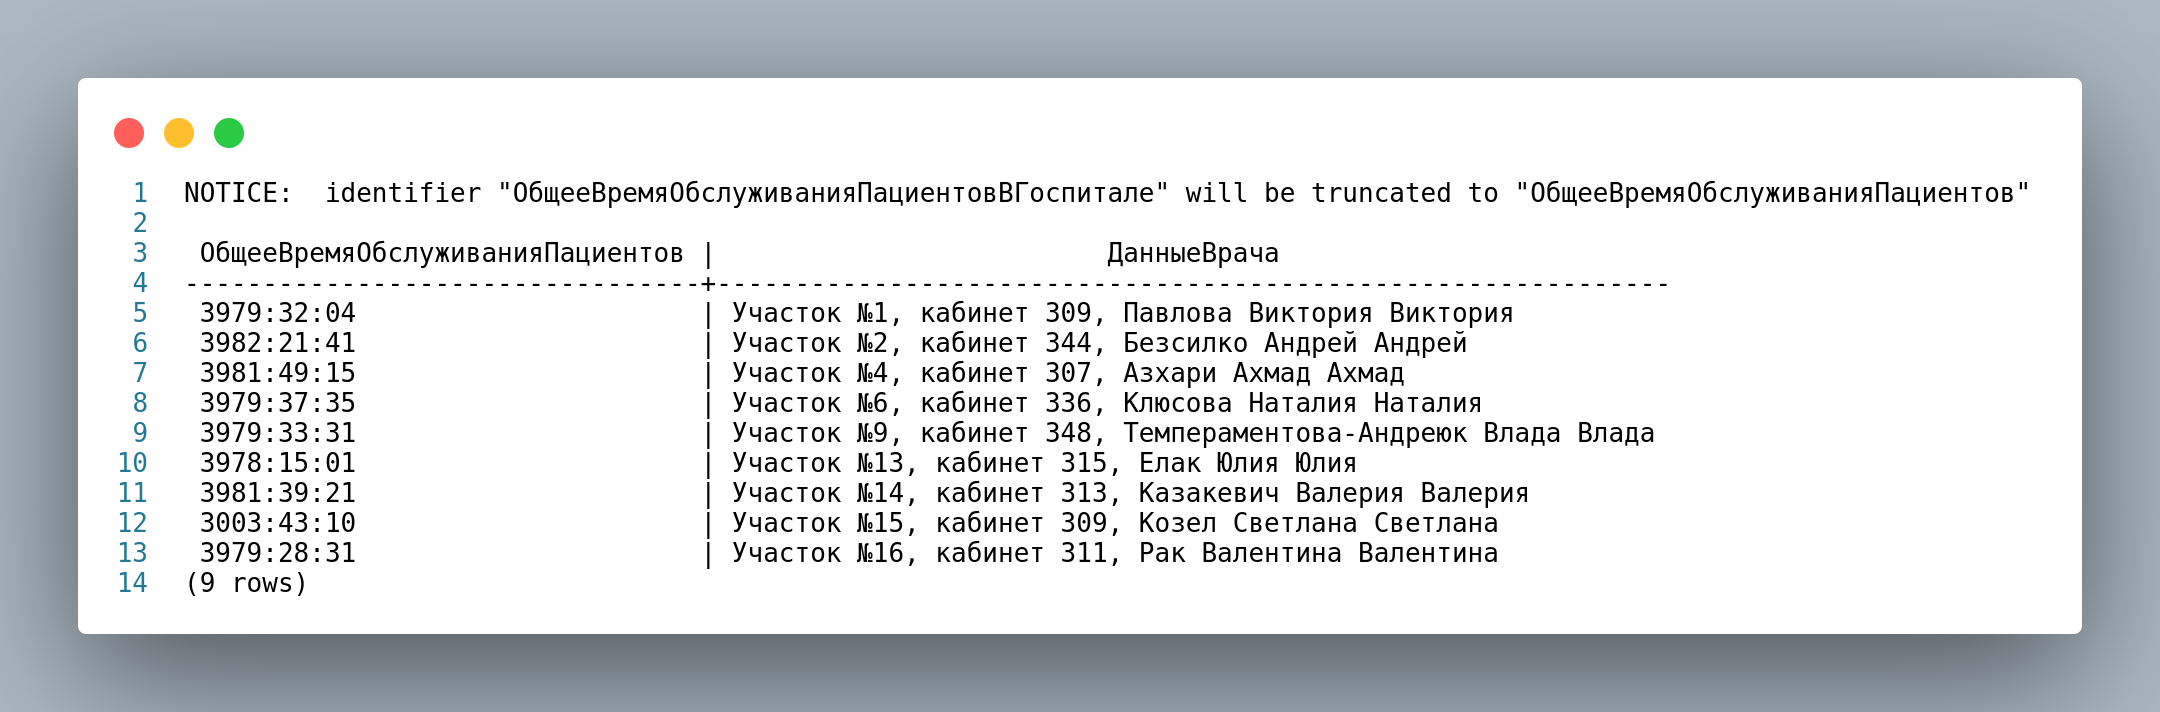
\includegraphics[width=18cm]
  {../sql/task4/4-out.png}

  \caption{Выборка из задания №4}

  \label{fig:t4}
\end{figure}

% = = = = = = = = = = = = = = = =

\begin{center}
  \textbf{Задание 5}
\end{center}
  
\textbf{Условие}:
Вывести диагнозы, которые не были поставлены ни одним врачом.
  
% \textbf{Что я сделал}:

% В таблице осмотры у меня 325632 осмотра. В таблице диагнозы у меня 14629 диагнозов.
% Из 325632 осмотра у меня за 3 года выявлено 14629 диагнозов, то есть все,
% поэтому я возьму обределённый период, например, 1 января 2019 - 20 февраля 2019.

% За два месяца (1 января 2019 - 20 февраля 2019) проведено 11734 осмотра и выявлено
% 7826 уникальных диагноза, тоесть не поставили диагнозов 6803 (14629-7826=6803).

% Из таблицы осмотры я вывел диагнозы от 1 января 2019 до 20 февраля 2019.

% Из таблицы диагнозы я отобрал те, которые были не поставлены от 1 января 2019 до 20 февраля 2019.

\lstinputlisting[language=sql]{../sql/task5/5.sql}

\textbf{Время выполнения}: 86-157 msec.

\textbf{Размер выборки}: 6424 rows.

\textbf{Результат}: часть выборки (в скриншоте LIMIT 48) изображена на рисунке~\ref{fig:t5}.

\begin{figure}[!h]
  \centering

  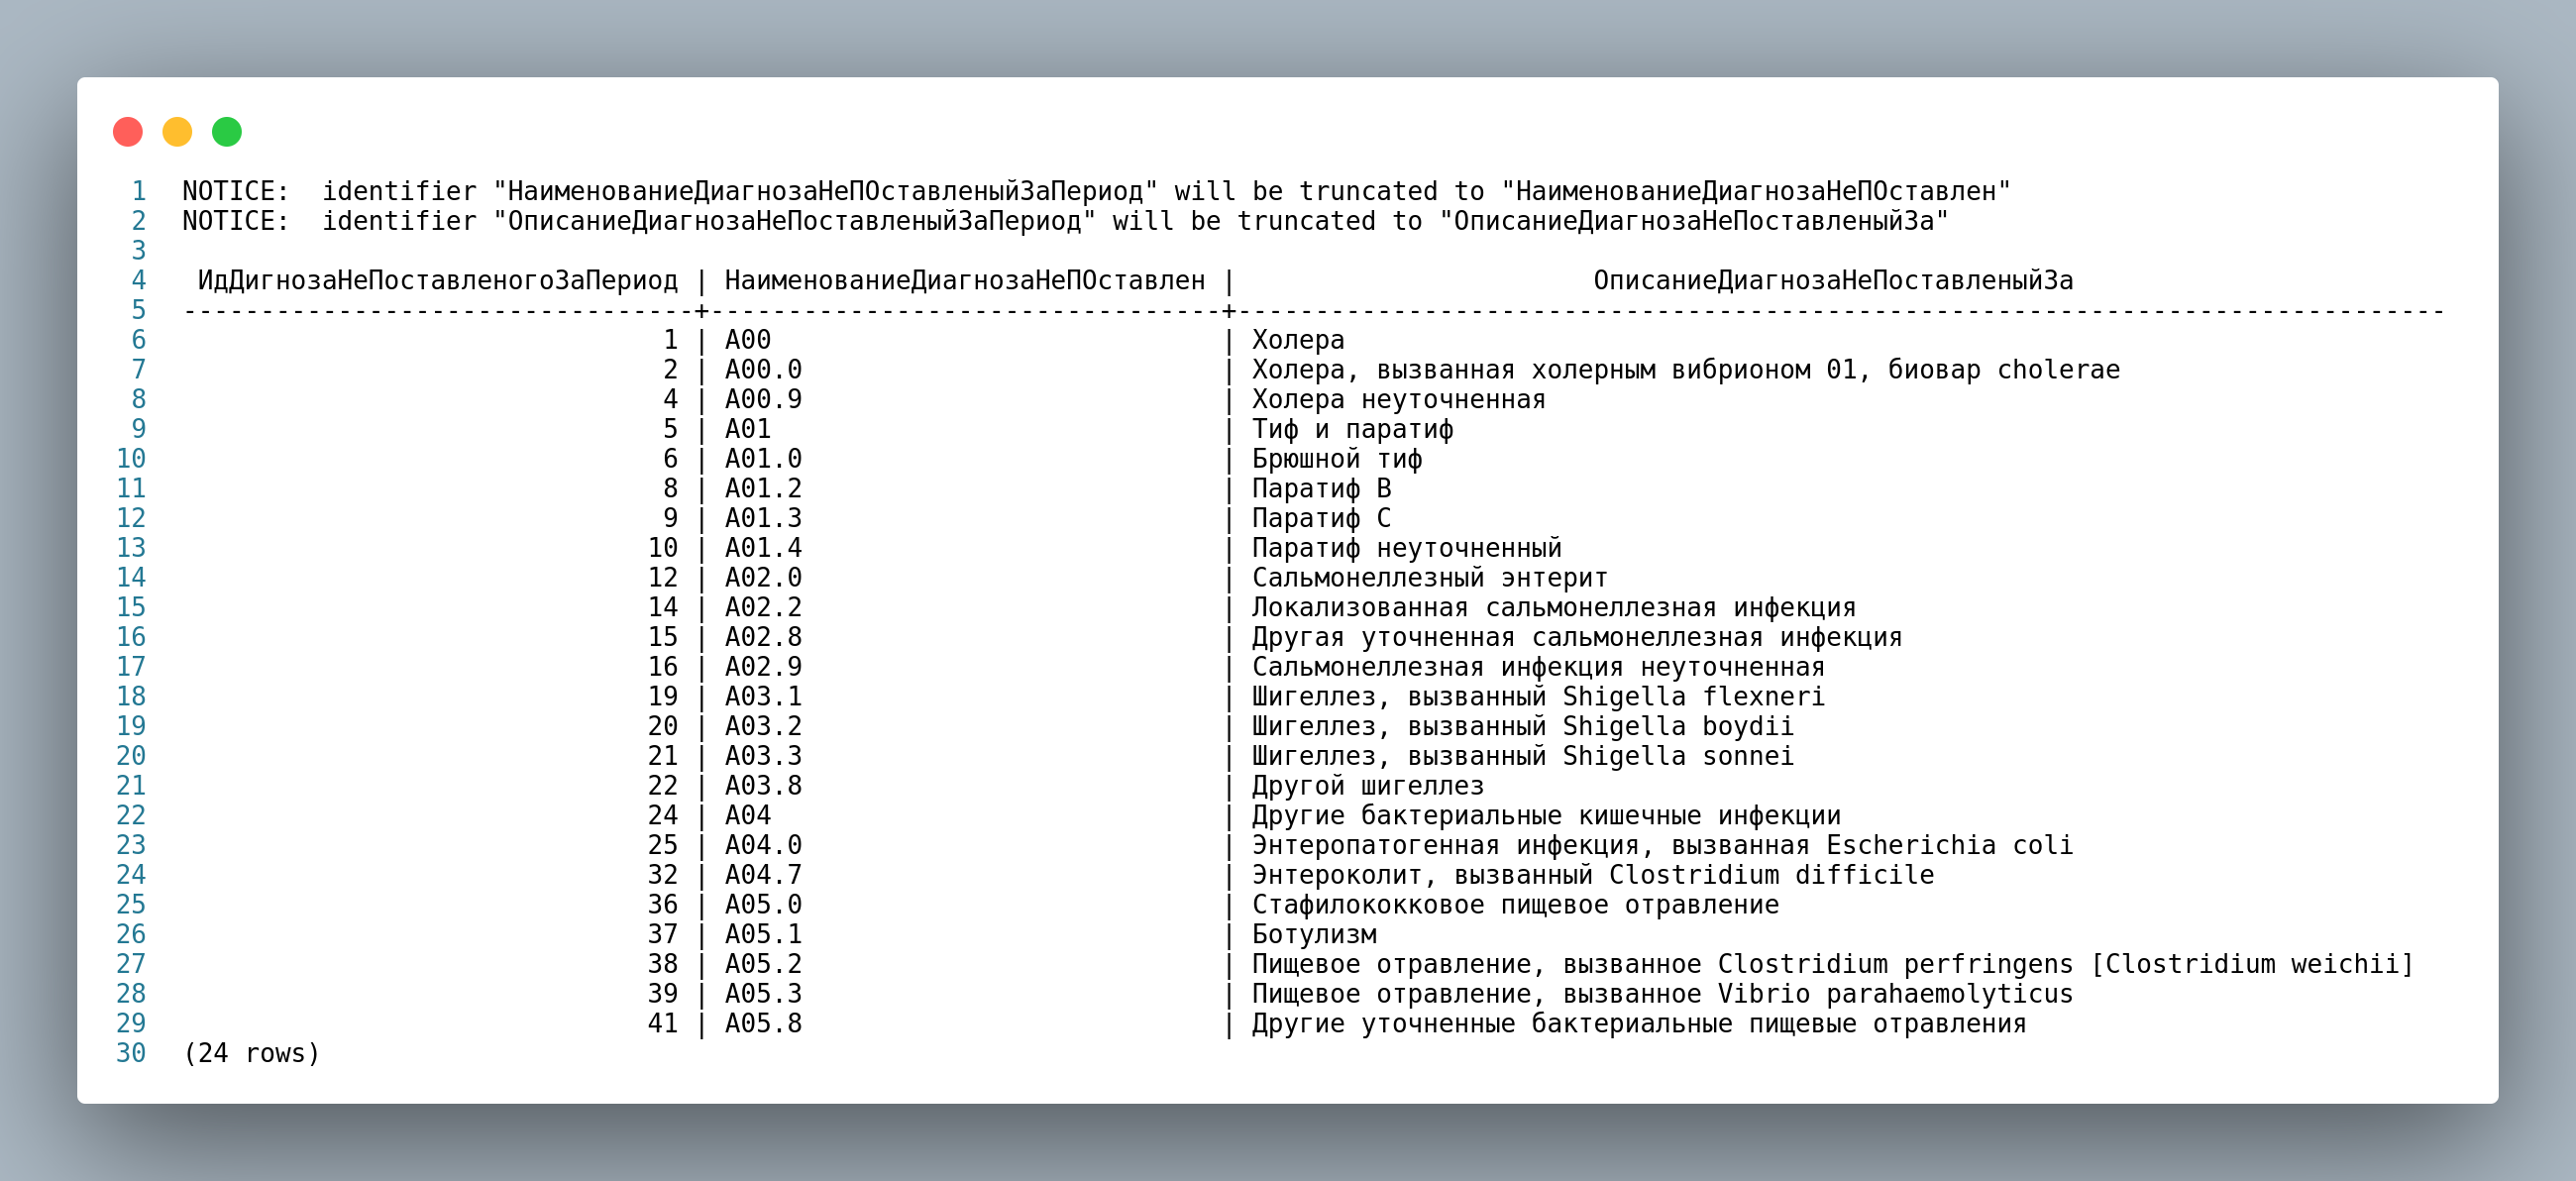
\includegraphics[width=18cm]
  {../sql/task5/5-out.png}

  \caption{Выборка из задания №5}

  \label{fig:t5}
\end{figure}

% = = = = = = = = = = = = = = = =

\begin{center}
  \textbf{Задание 6}
\end{center}
  
\textbf{Условие}:
В запросе для каждого врача подсчитать и вывести, начиная с даты 01.01.19, количество
пациентов каждого пола, а также количество пациентов, обслуженных не в госпитале
  
% \textbf{Что я сделал}:

% Объединил таблицы Осмотры-Пациенты, Пациенты-Гендеры, Осмотры-МестаОсмотра.

% Отобрал записи начиная от 1 января 2019 года.

% Сгруппировал записи по гендору пациента и месту осмотра.

\lstinputlisting[language=sql]{../sql/task6/6.sql}

\textbf{Время выполнения}: 249-325 msec.

\textbf{Размер выборки}: 56 rows.

\textbf{Результат}: вся выборка изображена на рисунке~\ref{fig:t6}.

\begin{figure}[!h]
  \centering

  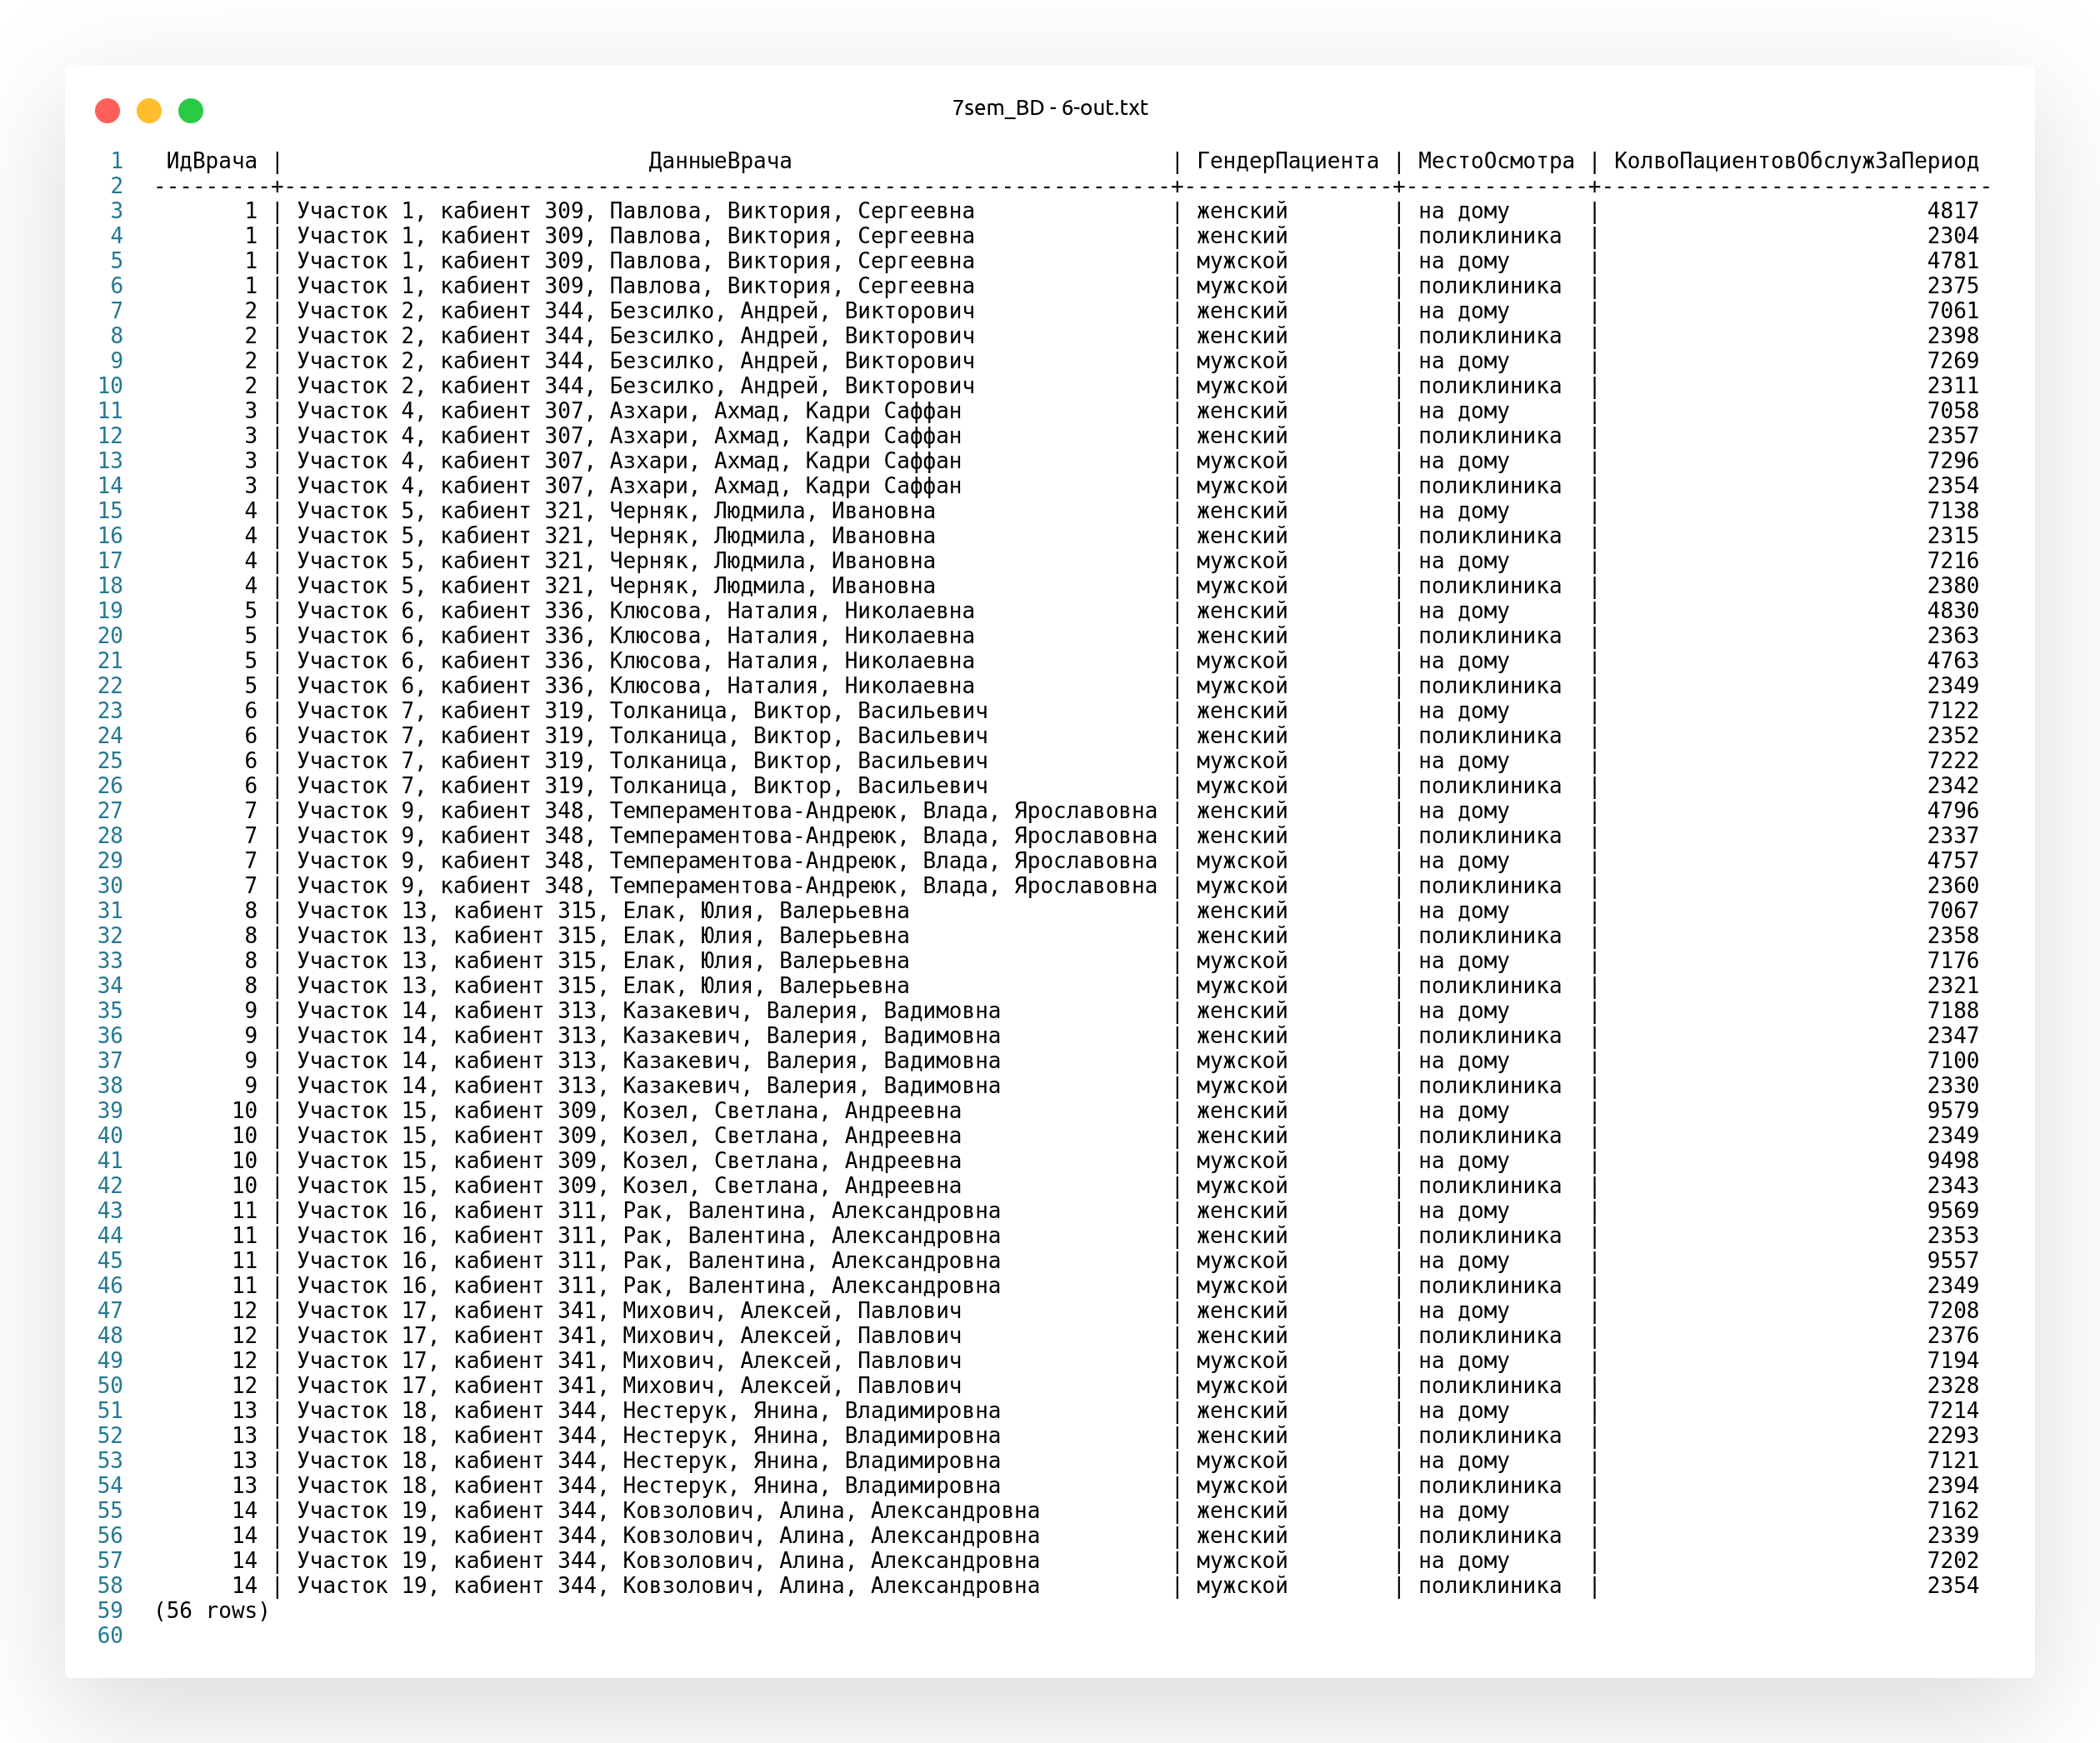
\includegraphics[width=18cm]
  {../sql/task6/6-out.png}

  \caption{Выборка из задания №6}

  \label{fig:t6}
\end{figure}

% = = = = = = = = = = = = = = = =

\begin{center}
  \textbf{Задание 7}
\end{center}
  
\textbf{Условие}:
Написать запрос, выводящий для каждого диагноза количество пациентов, название
самого диагноза, а также средний возраст пациентов диагноза

% \textbf{Что я сделал}:

% Я объединил таблицы Осмотры-Пациенты, Осмотры-Диагнозы.

% Я сгруппировал выборку по ид дигноза.

% Я подсчитал количество каждого дигноза отдельно.

% Я подсчитал средний возвраст для каждого диагноза.

\lstinputlisting[language=sql]{../sql/task7/7.sql}

\textbf{Время выполнения}: 792-868 msec.

\textbf{Размер выборки}: 14629 rows.

\textbf{Результат}: часть выборки (в скриншоте LIMIT 48) изображена на рисунке~\ref{fig:t7}.

\begin{figure}[!h]
  \centering

  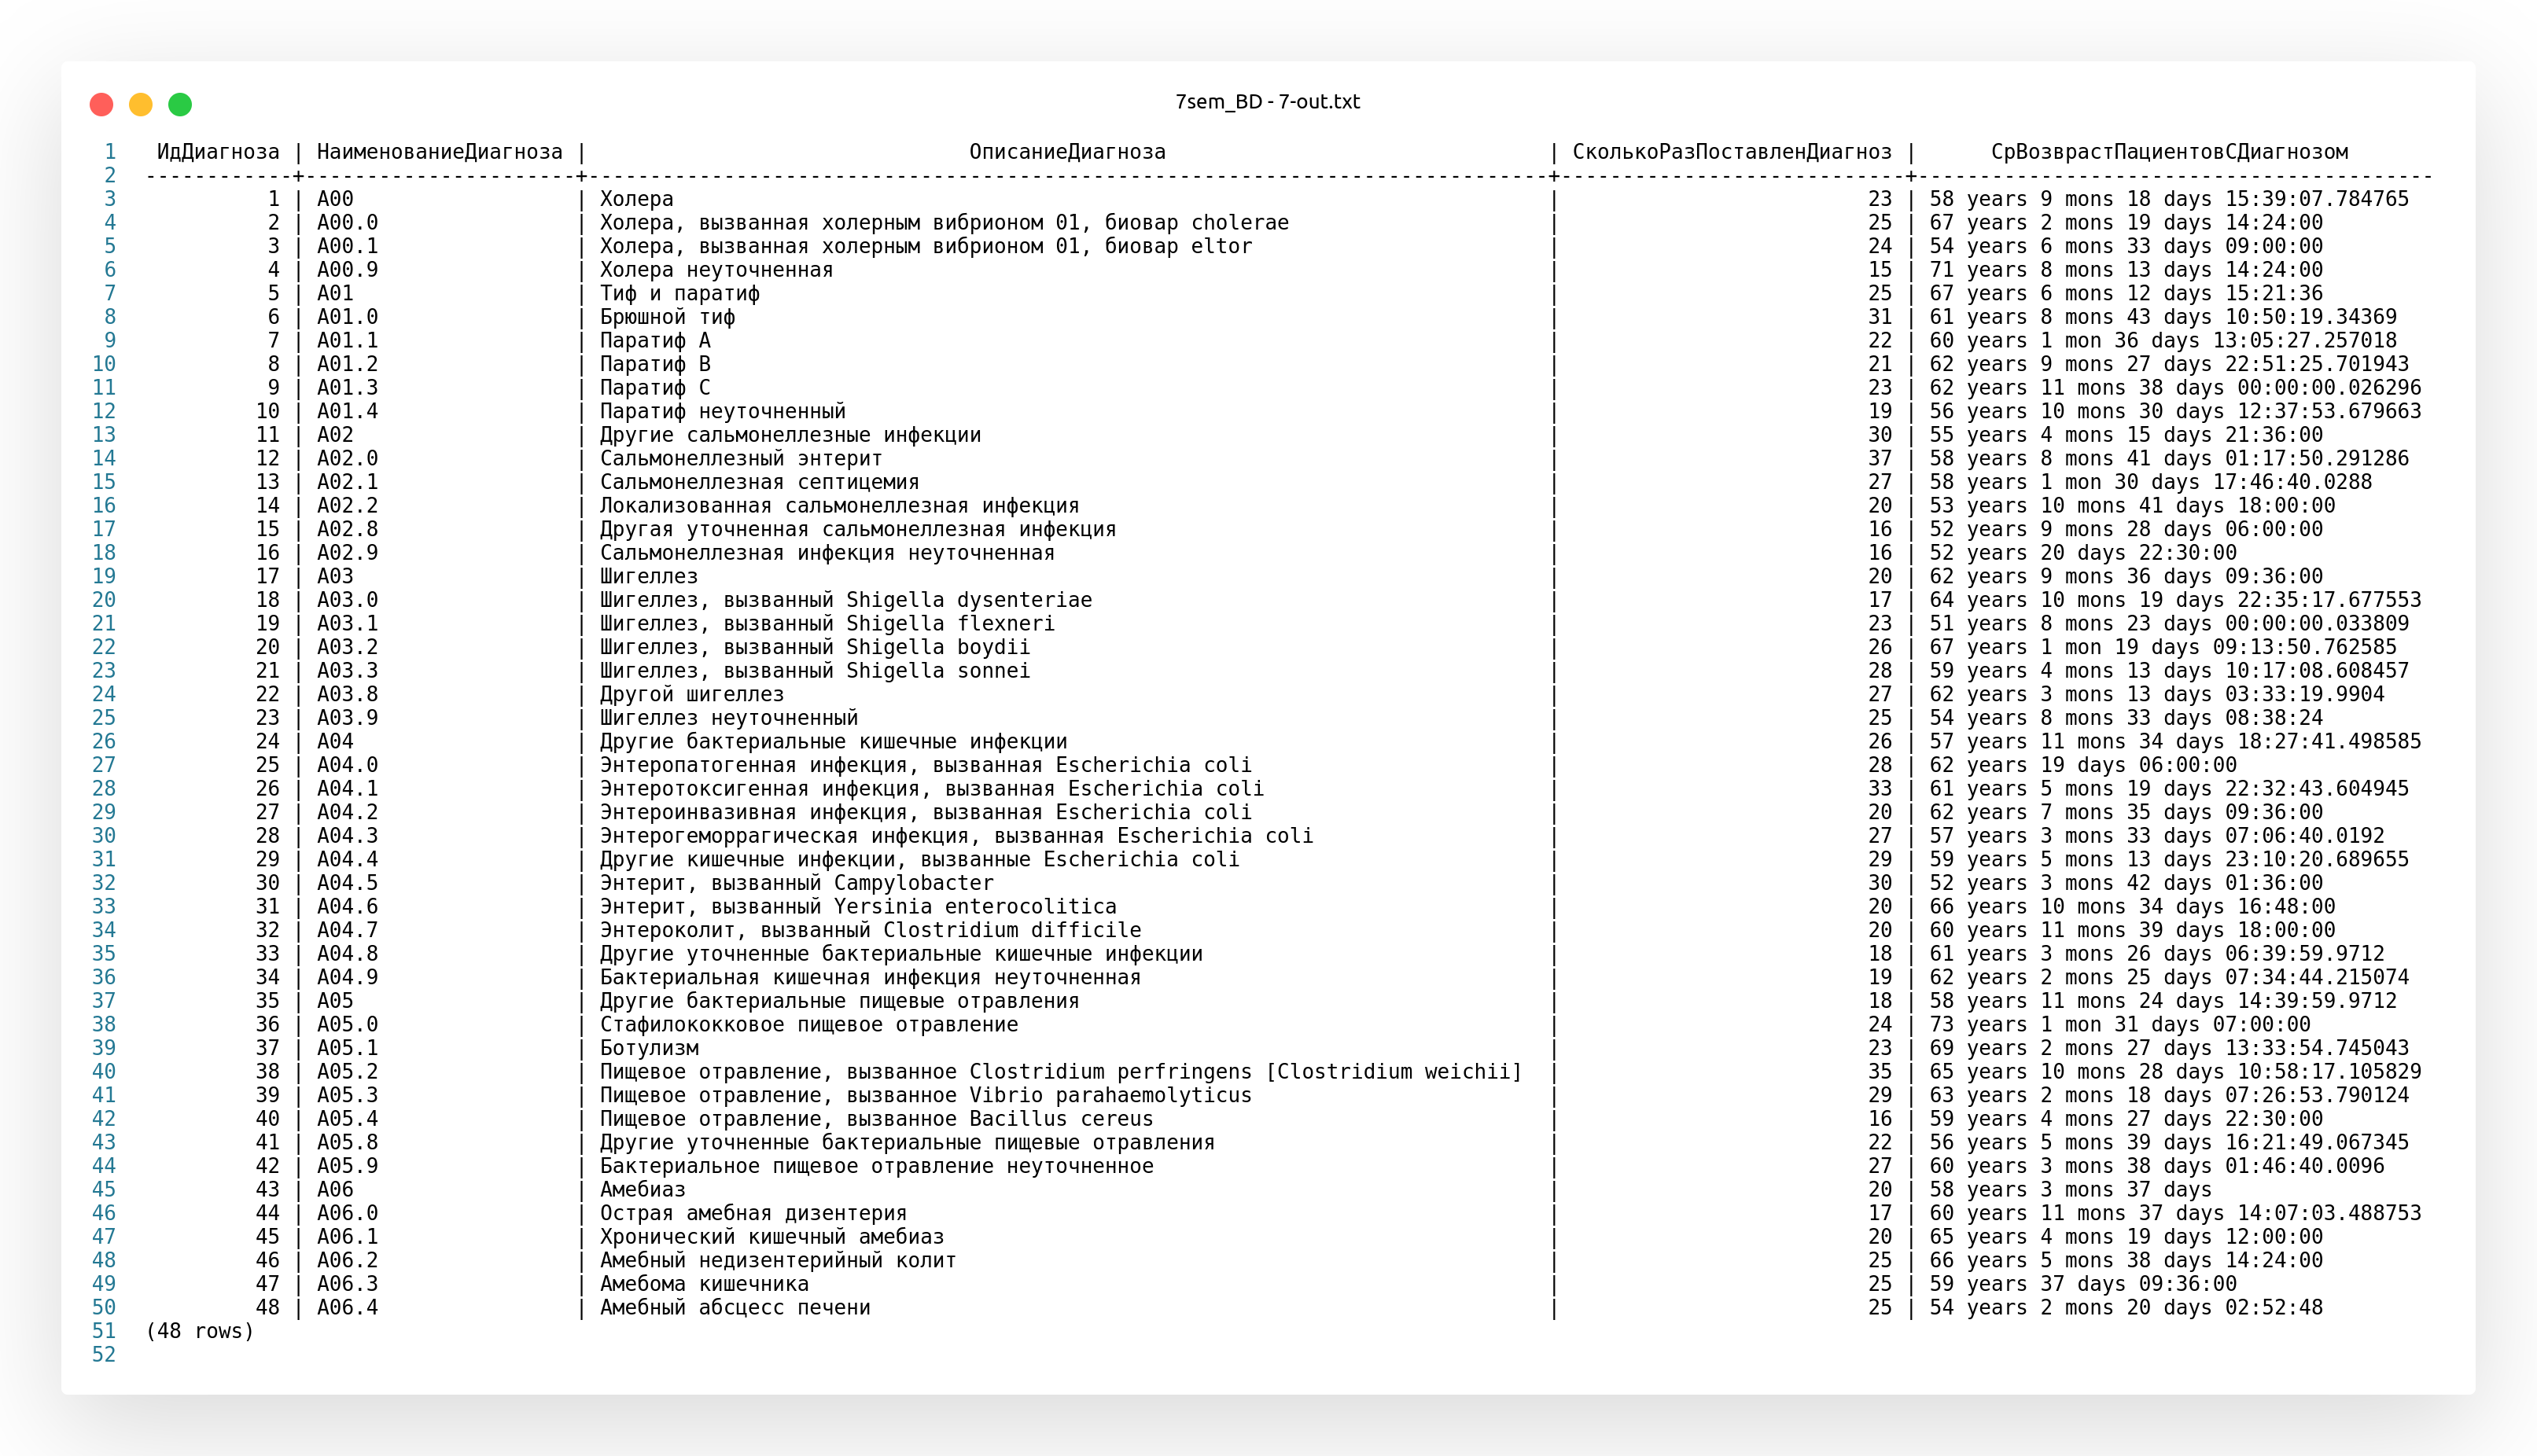
\includegraphics[width=18cm]
  {../sql/task7/7-out.png}

  \caption{Выборка из задания №7}

  \label{fig:t7}
\end{figure}

\newpage

% = = = = = = = = = = = = = = = =

\begin{center}
  \textbf{Задание 8}
\end{center}
  
\textbf{Условие}:
Вывести данные о врачах, у которых существует хотя бы один пациент старше 100 лет.

% \textbf{Что я сделал}:

% Я соединил таблицы Осмотры-Пациенты, Осмотры-Врачи.

% Я отобрал записи, у которых пациент имеет больше 100 лет.

% Я вывел сконкатенированные данные о враче.

% Я вывел сконкатенированные данные о пациенте.

\lstinputlisting[language=sql]{../sql/task8/8.sql}

\textbf{Время выполнения}: 174-230 msec.

\textbf{Размер выборки}: 464 rows.

\textbf{Результат}: часть выборки (в скриншоте LIMIT 48) изображена на рисунке~\ref{fig:t8}.

\begin{figure}[!h]
  \centering

  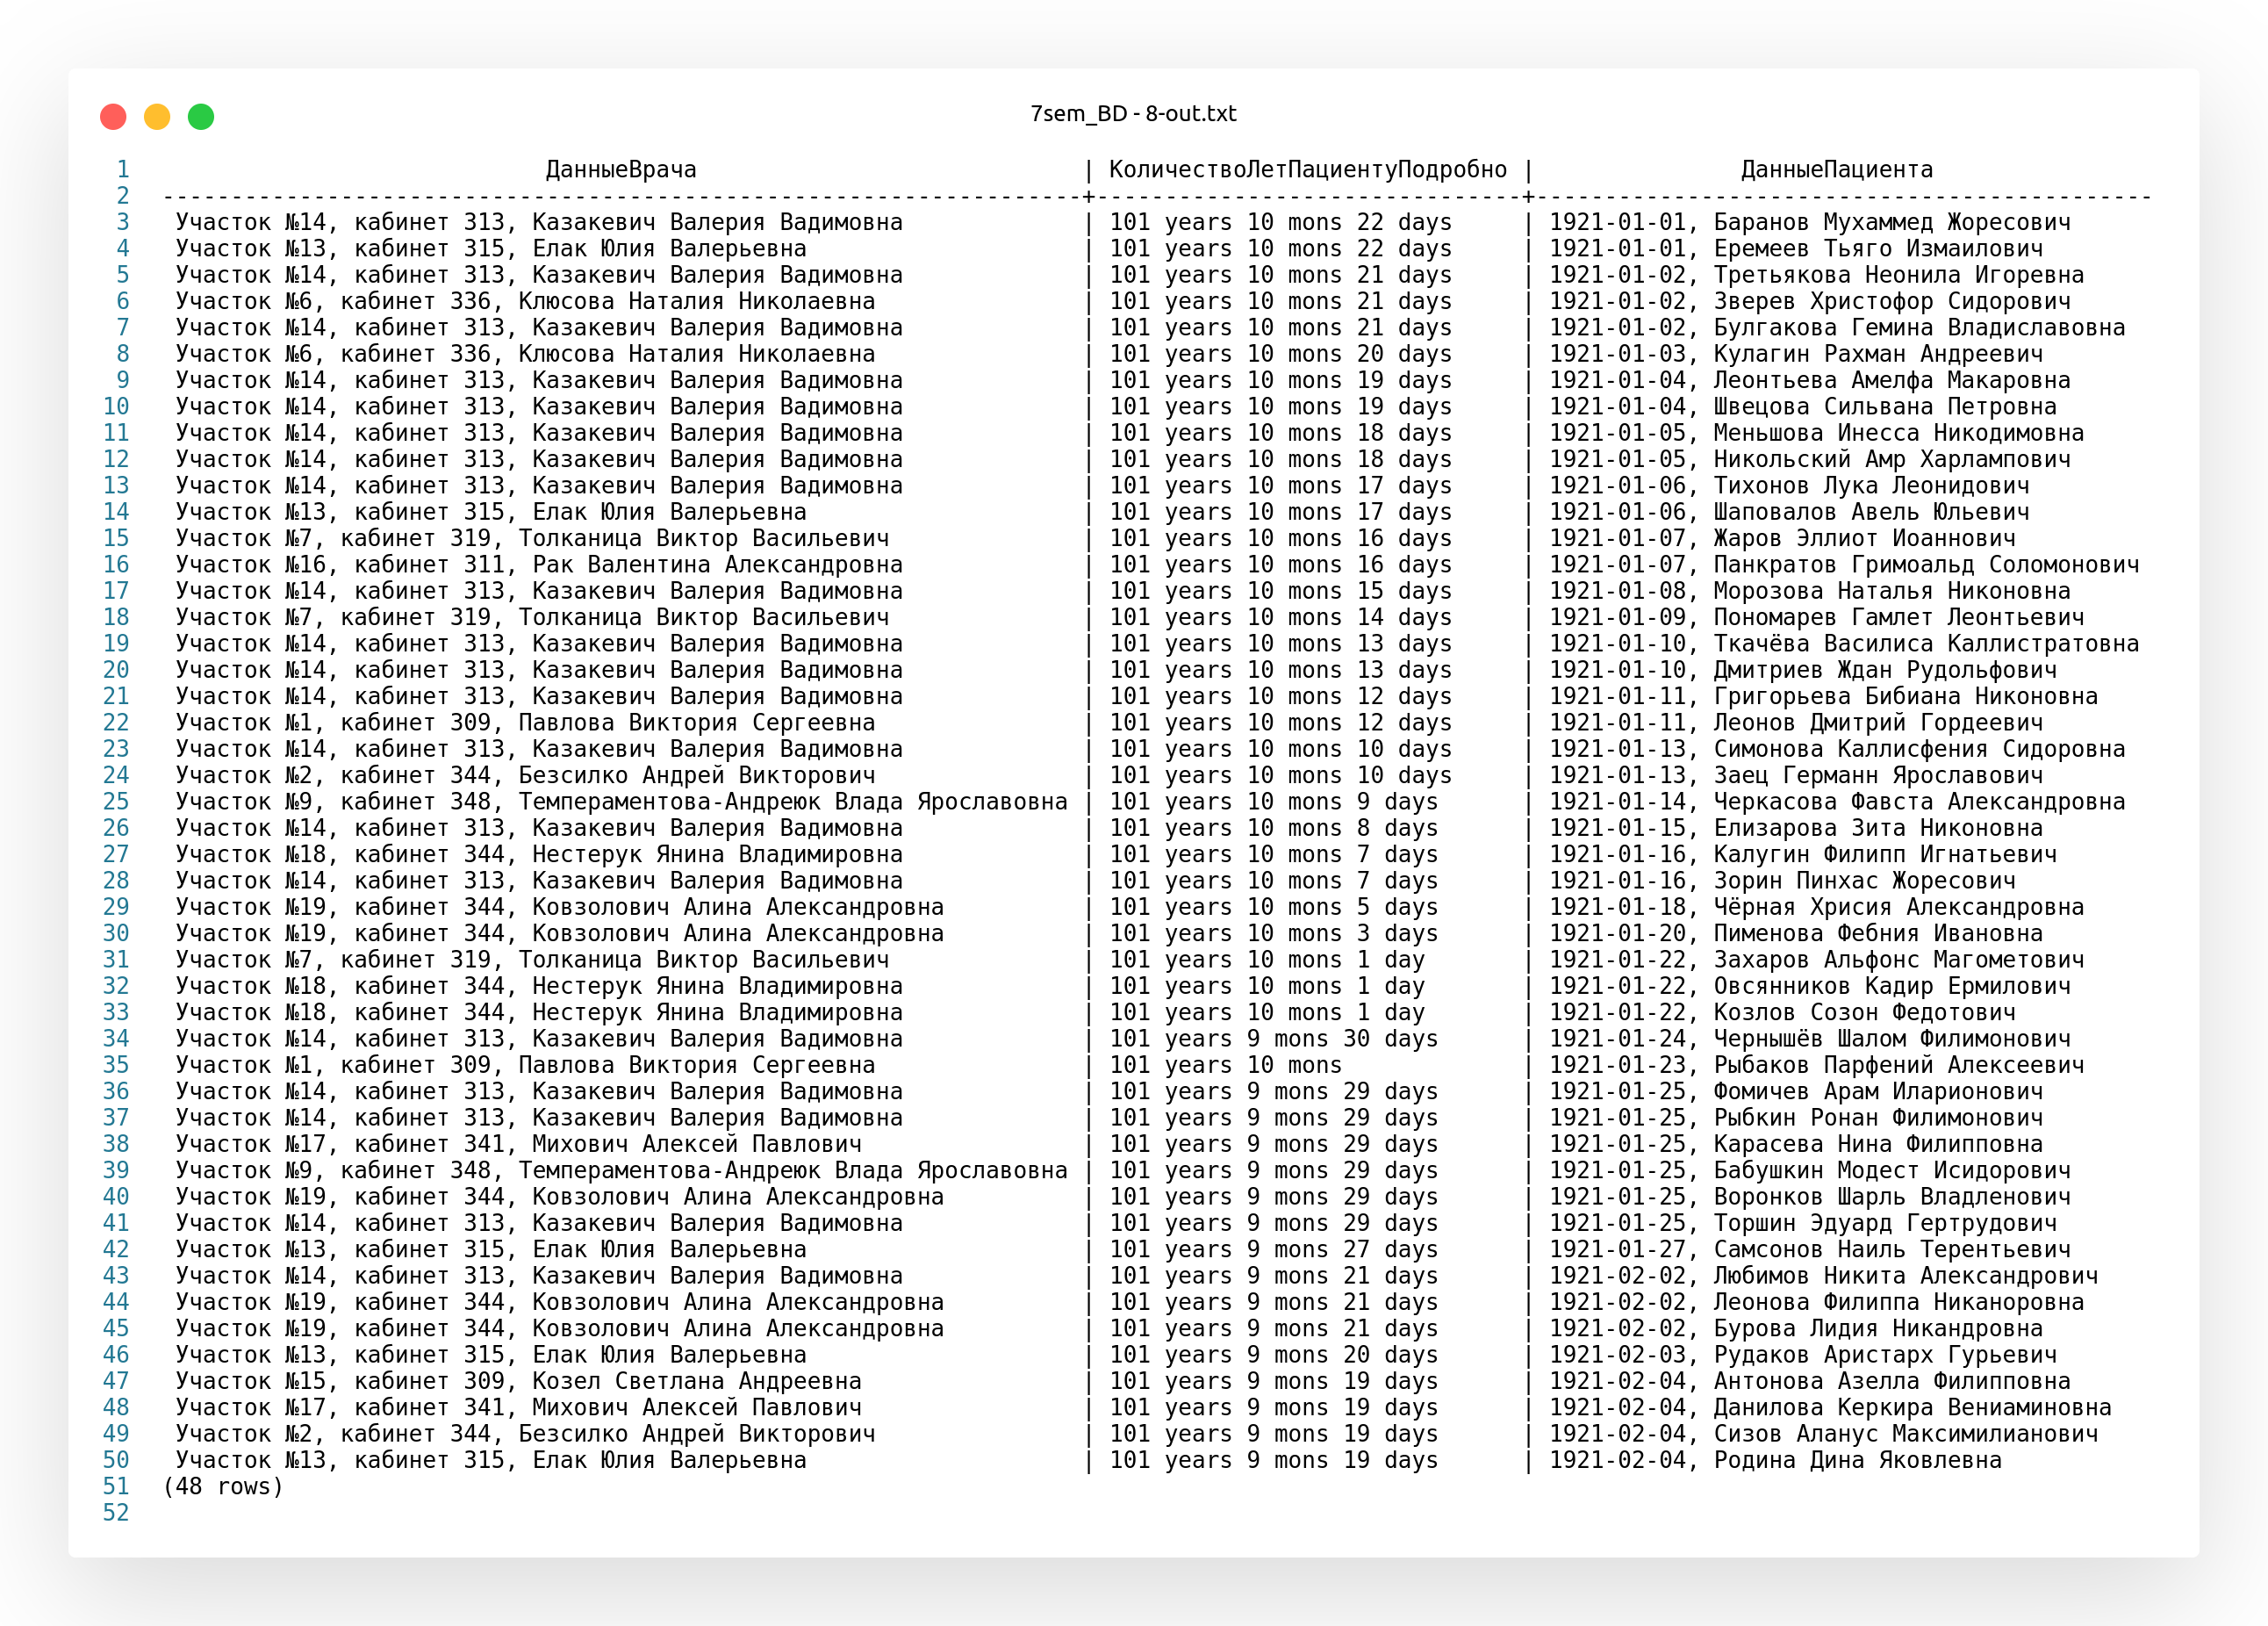
\includegraphics[width=18cm]
  {../sql/task8/8-out.png}

  \caption{Выборка из задания №8}

  \label{fig:t8}
\end{figure}

% = = = = = = = = = = = = = = = =

\newpage

\begin{center}
  \textbf{Задание 9}
\end{center}
  
\textbf{Условие}:
Вывести данные о самых молодых пациентах, которым прописано максимальное
количество лекарств.

% \textbf{Что я сделал}:

% Я нашел минимальный возвраст пациента в подзапросе.

% Я сгруппировал записи по ид пациента и нашел количество выписанных лекарств для каждого пациента.

% Я нашел максимальное количество лекарств у молодого пациента в подзапросе.

% Я сконкатенировал данные пациента.

\lstinputlisting[language=sql]{../sql/task9/9.sql}

\textbf{Время выполнения}: 859-981 msec.

\textbf{Размер выборки}: 90 row.

\textbf{Результат}: вся выборка изображена на рисунке~\ref{fig:t9}.

\begin{figure}[!h]
  \centering

  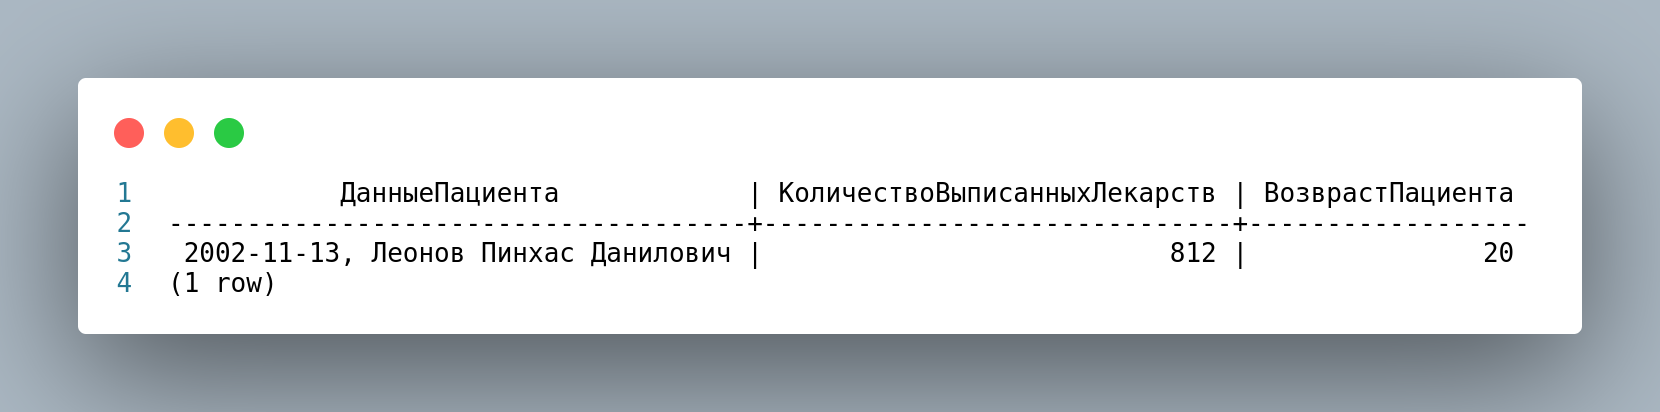
\includegraphics[width=18cm]
  {../sql/task9/9-out.png}

  \caption{Выборка из задания №9}

  \label{fig:t9}
\end{figure}

\newpage

% = = = = = = = = = = = = = = = =

\begin{center}
  \textbf{Задание 10}
\end{center}
  
\textbf{Условие}:
Вывести данные о пациентах, о которых точно известно, что они никогда не обслуживались дома.

% \textbf{Что я сделал}:

% Я соединил таблицы Осмотры-МестаОсомтра в подзапросе.

% В подзапросе я отобрал записи осмотра на дому.

% Взяв таблицу пациентов, я высек тех пациентов, которые обслуживались дома, то есть оставив тех, кто дома не обслуживался. 

\lstinputlisting[language=sql]{../sql/task10/10.sql}

\textbf{Время выполнения}: 152-213 msec.

\textbf{Размер выборки}: 11494 rows.

\textbf{Результат}: часть выборки (в скриншоте LIMIT 48) изображена на рисунке~\ref{fig:t10}.

\begin{figure}[!h]
  \centering

  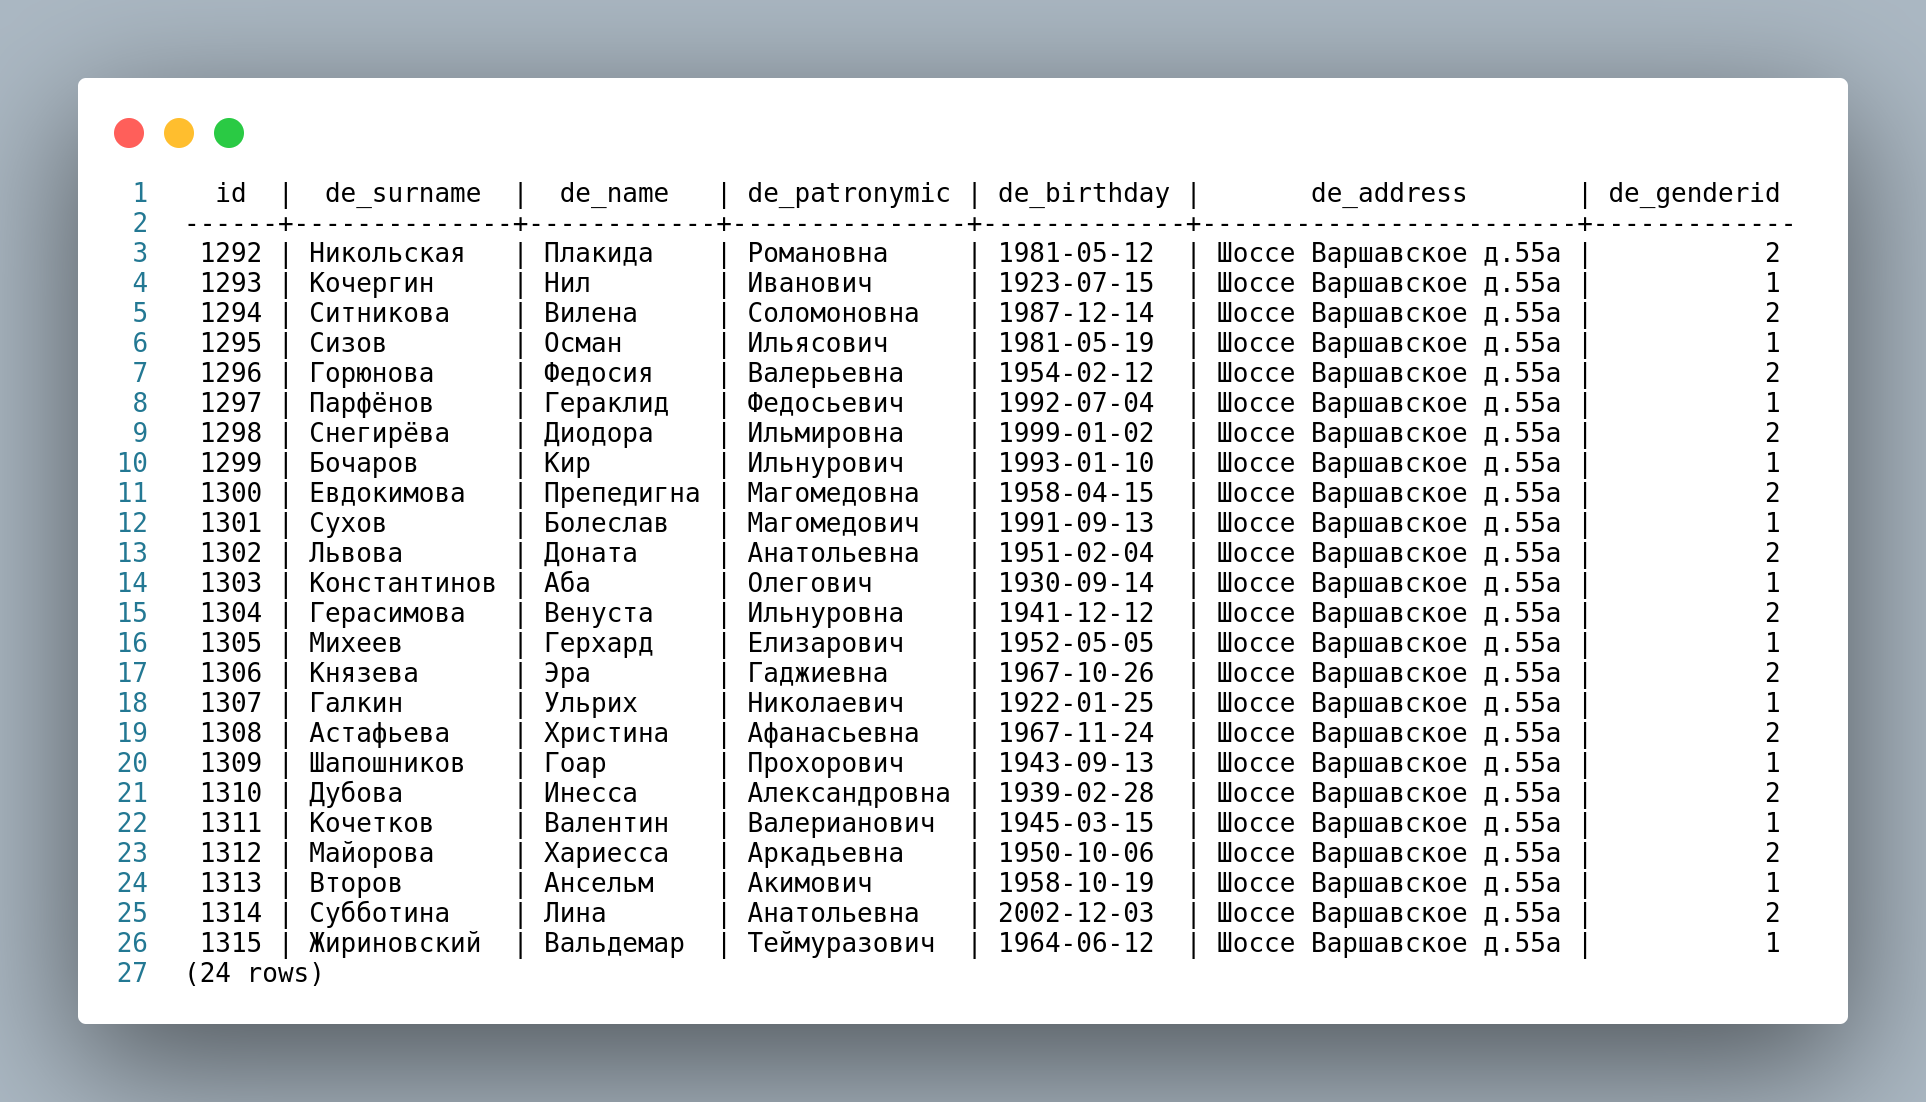
\includegraphics[width=18cm]
  {../sql/task10/10-out.png}

  \caption{Выборка из задания №10}

  \label{fig:t10}
\end{figure}

\newpage

% = = = = = = = = = = = = = = = =

\begin{center}
  \textbf{Задание 11}
\end{center}
  
\textbf{Условие}:
Для каждого врача вывести в минутах среднее время приёма, данные отсортировать по
убыванию значений среднего времени приема

% \textbf{Что я сделал}:

\lstinputlisting[language=sql]{../sql/task11/11.sql}

\textbf{Время выполнения}: 310-378 msec.

\textbf{Размер выборки}: 28 rows.

\textbf{Результат}: вся выборка изображена на рисунке~\ref{fig:t11}.

\begin{figure}[!h]
  \centering

  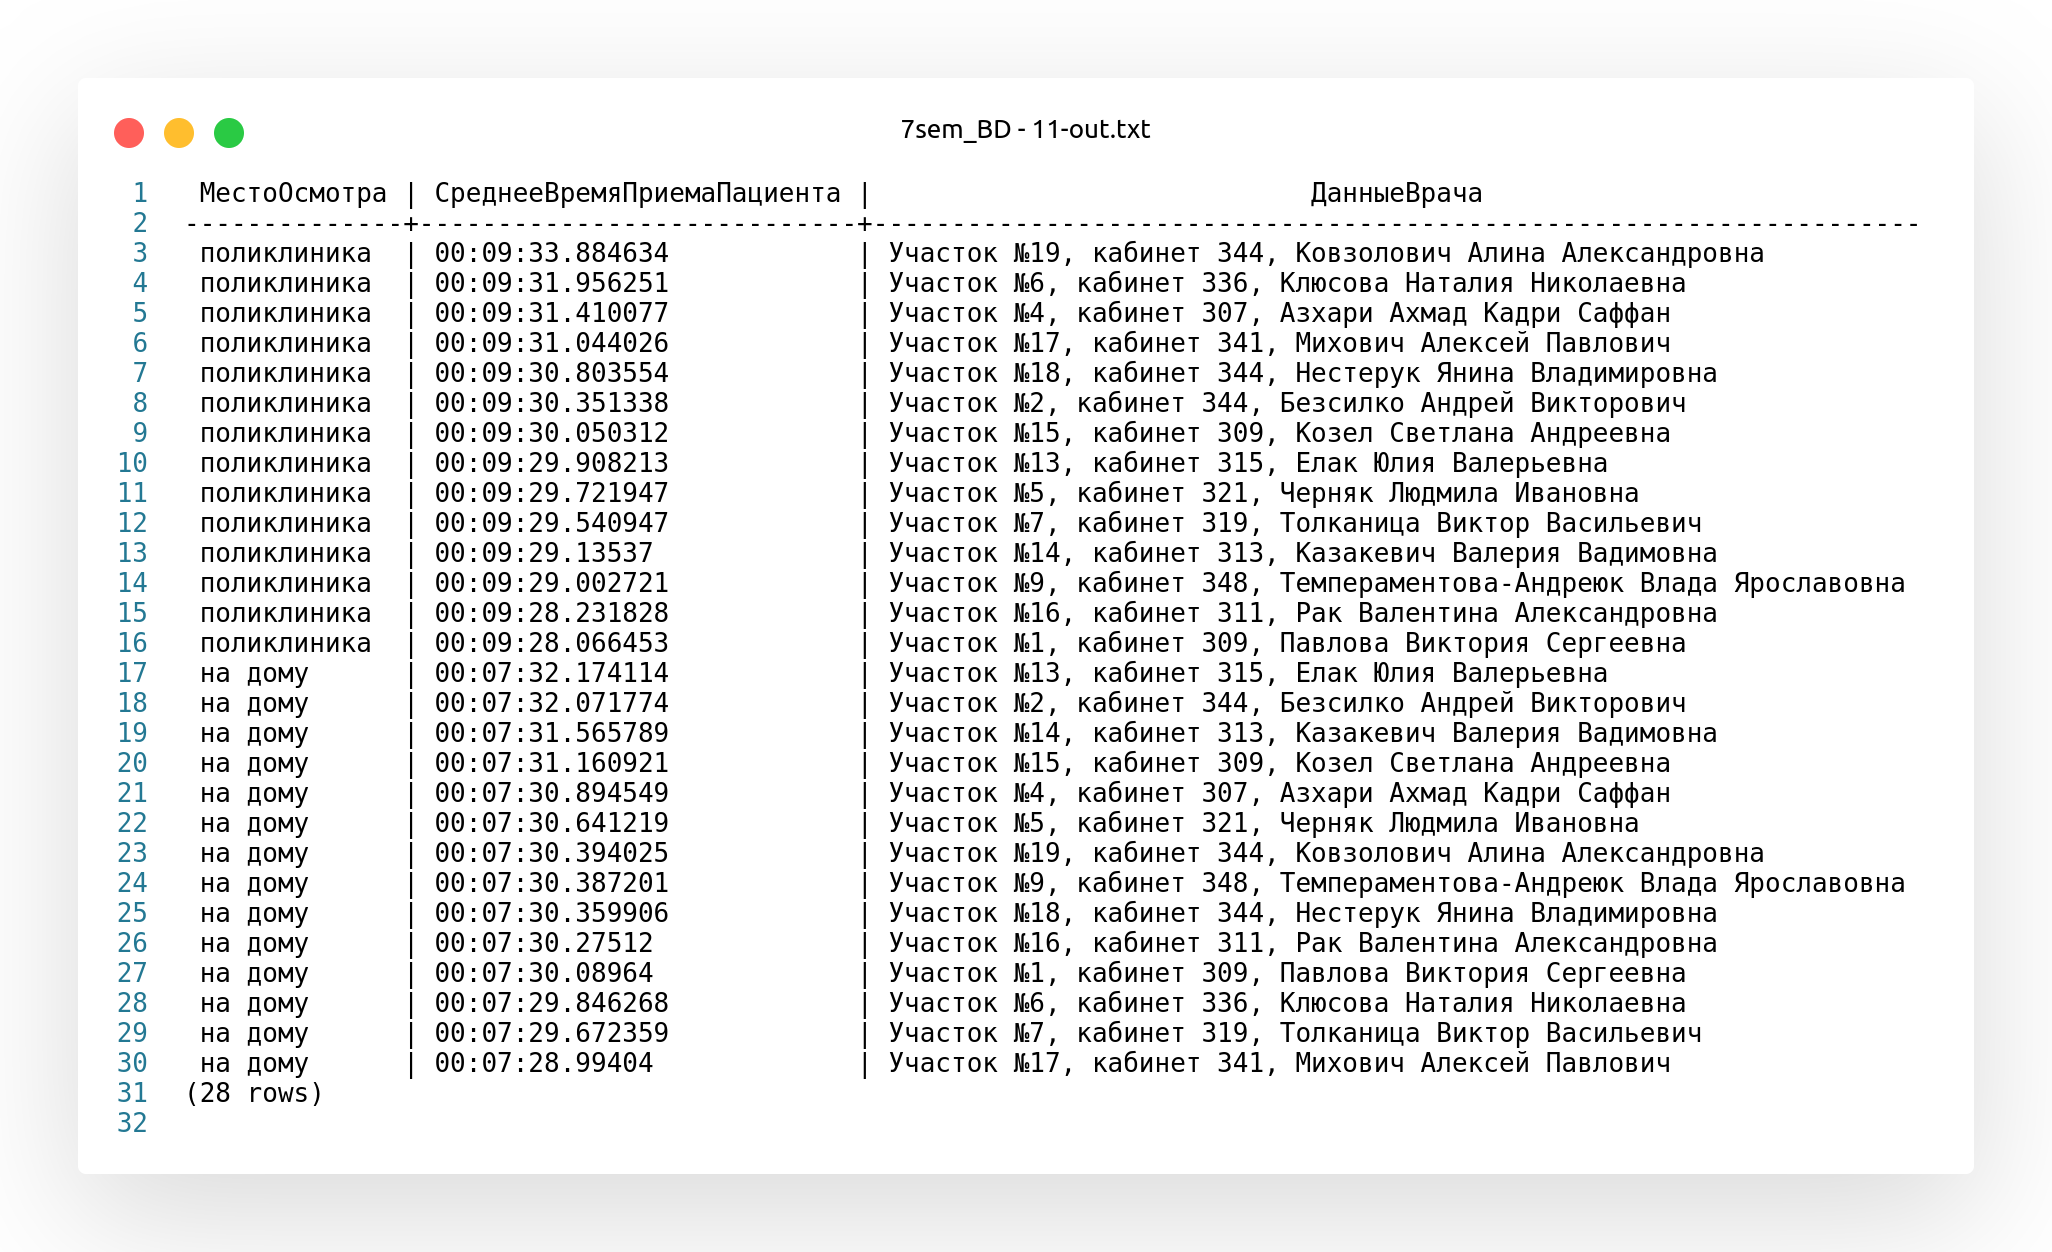
\includegraphics[width=18cm]
  {../sql/task11/11-out.png}

  \caption{Выборка из задания №11}

  \label{fig:t11}
\end{figure}

% = = = = = = = = = = = = = = = =

\newpage

\begin{center}
  \textbf{Задание 12}
\end{center}
  
\textbf{Условие}:
Вывести минимальный интервал между обращениями одного и того же пациента к врачу,
а также данные пациента и врача

\lstinputlisting[language=sql]{../sql/task12/12.sql}

\textbf{Время выполнения}: 78-168 msec.

\textbf{Размер выборки}: 2081 rows.

\textbf{Результат}: часть выборки (в скриншоте LIMIT 48) изображена на рисунке~\ref{fig:t12}.

\begin{figure}[!h]
  \centering

  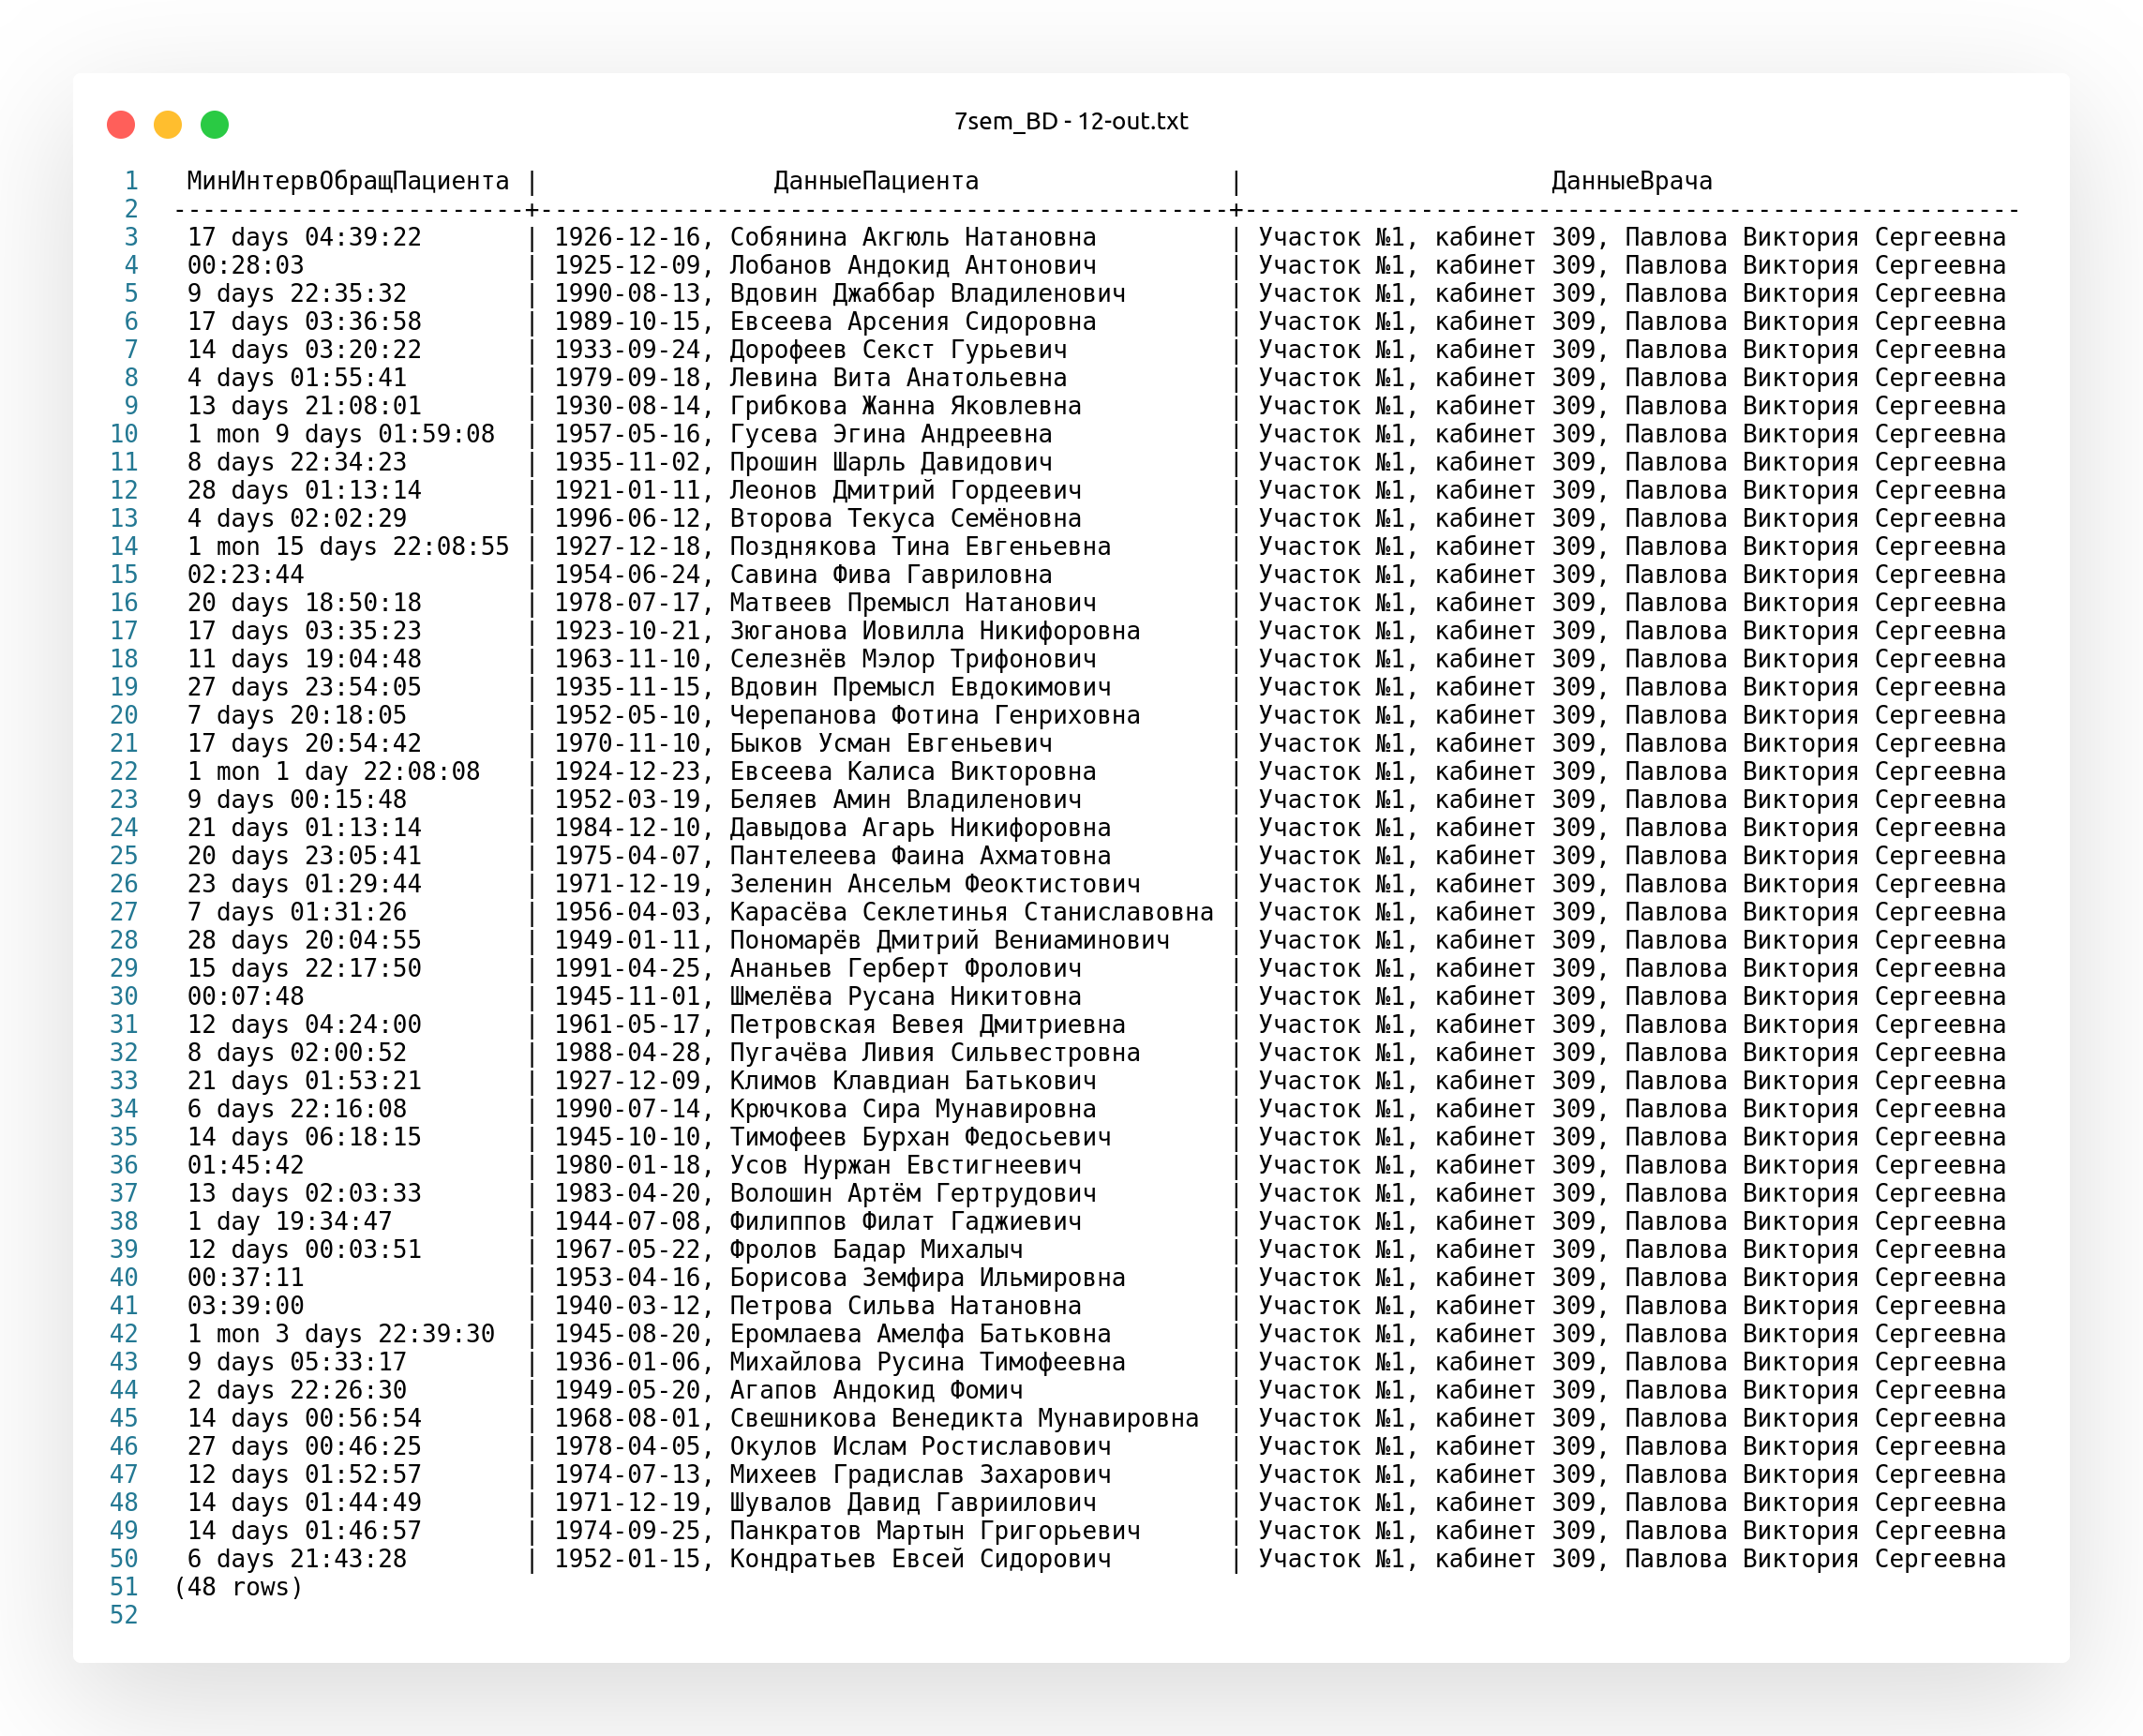
\includegraphics[width=18cm]
  {../sql/task12/12-out.png}

  \caption{Выборка из задания №12}

  \label{fig:t12}
\end{figure}

% = = = = = = = = = = = = = = = =

\newpage

\begin{center}
  \textbf{Задание 13}
\end{center}
  
\textbf{Условие}:
Вывести данные врача, поставившего все диагнозы, которые присутствуют в базе данных

\lstinputlisting[language=sql]{../sql/task13/13.sql}

\textbf{Время выполнения}: 188-253 msec.

\textbf{Размер выборки}: 14 rows.

\textbf{Результат}: вся выборка изображена на рисунке~\ref{fig:t13}.

\begin{figure}[!h]
  \centering

  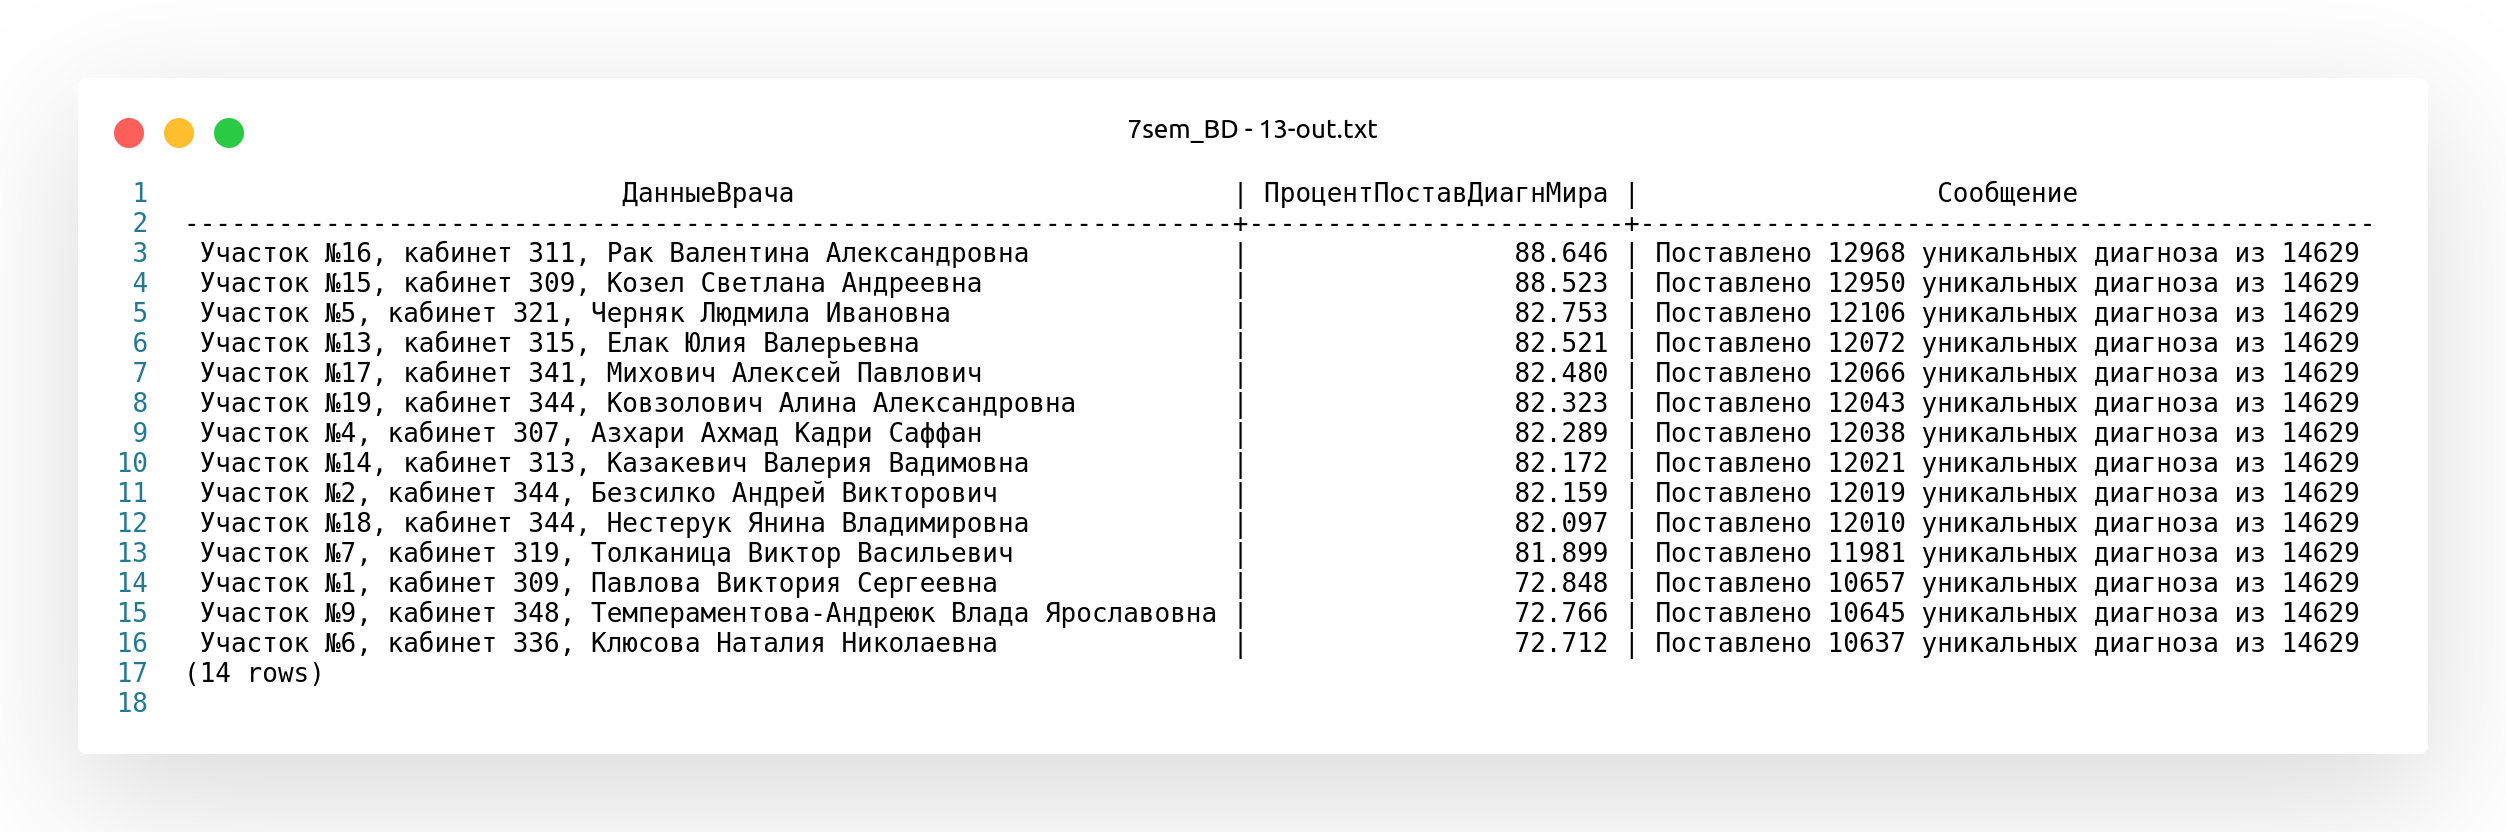
\includegraphics[width=18cm]
  {../sql/task13/13-out.png}

  \caption{Выборка из задания №13}

  \label{fig:t13}
\end{figure}

% = = = = = = = = = = = = = = = =

\newpage

\begin{center}
  \textbf{Задание 14}
\end{center}
  
\textbf{Условие}:
Вывести данные обо всех пациентах и количестве выписанных им лекарств, которым
выписаны суммарно лекарств больше, чем выписано лекарств пациенту Иванову И.И.

\lstinputlisting[language=sql]{../sql/task14/14.sql}

\textbf{Время выполнения}: 6 sec 86 msec - 6 sec 445 msec.

\textbf{Размер выборки}: 4144 rows.

\textbf{Результат}: вся выборка изображена на рисунке~\ref{fig:t14}.

\begin{figure}[!h]
  \centering

  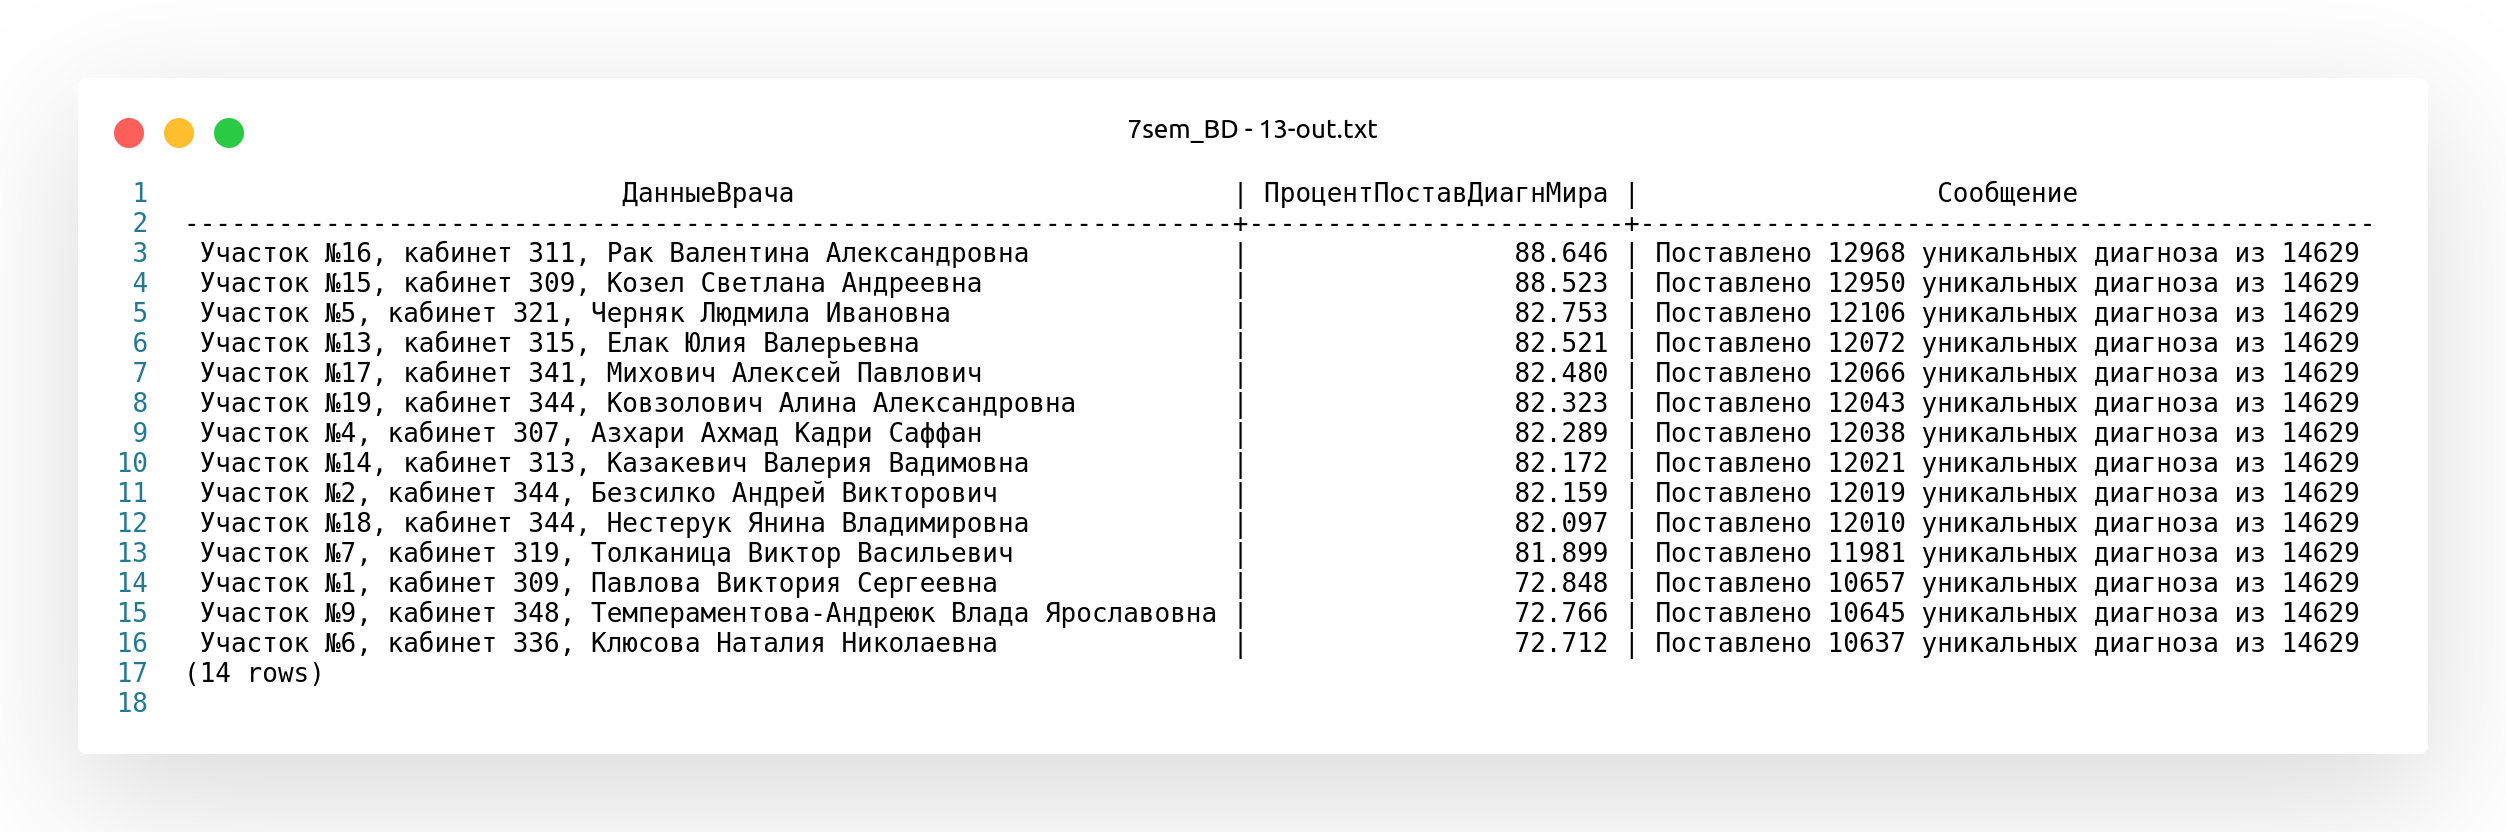
\includegraphics[height=4.5cm]
  {../sql/task13/13-out.png}

  \caption{Выборка из задания №14}

  \label{fig:t14}
\end{figure}

% = = = = = = = = = = = = = = = =

\newpage

\begin{center}
  \textbf{Задание 15}
\end{center}
  
\textbf{Условие}:
Вывести данные обо всех пациентах, количестве выписанных им лекарств, которые имеют
абсолютно точно такие же диагнозы, что и пациент Иванов И.И.

% \lstinputlisting[language=sql]{../sql/task15/15.sql}

\newpage
